\documentclass[a4paper,12pt,twoside,openany]{report}
%
% Wzorzec pracy dyplomowej
% J. Starzynski (jstar@iem.pw.edu.pl) na podstawie pracy dyplomowej
% mgr. inż. Błażeja Wincenciaka
% Wersja 0.1 - 8 października 2016
%
\usepackage{polski}
\usepackage{helvet}
\usepackage[T1]{fontenc}
\usepackage{anyfontsize}
\usepackage[utf8]{inputenc}
\usepackage[pdftex]{graphicx}
\usepackage{tabularx}
\usepackage{array}
\usepackage[polish]{babel}
\usepackage{subfigure}
\usepackage{amsfonts}
\usepackage{verbatim}
\usepackage{indentfirst}
\usepackage[pdftex]{hyperref}


% rozmaite polecenia pomocnicze
% gdzie rysunki?
\newcommand{\ImgPath}{.}

% oznaczenie rzeczy do zrobienia/poprawienia
\newcommand{\TODO}{\textbf{TODO}}


% wyroznienie slow kluczowych
\newcommand{\tech}{\texttt}

% na oprawe (1.0cm - 0.7cm)*2 = 0.6cm
% na oprawe (1.1cm - 0.7cm)*2 = 0.8cm
%  oddsidemargin lewy margines na nieparzystych stronach
% evensidemargin lewy margines na parzystych stronach
\def\oprawa{1.05cm}
\addtolength{\oddsidemargin}{\oprawa}
\addtolength{\evensidemargin}{-\oprawa}

% table span multirows
\usepackage{multirow}
\usepackage{enumitem}	% enumitem.pdf
\setlist{listparindent=\parindent, parsep=\parskip} % potrzebuje enumitem

%%%%%%%%%%%%%%% [nazarewk] Z templatki pandoc %%%%%%%%%%%%%%%%
\providecommand{\tightlist}{%
  \setlength{\itemsep}{0pt}\setlength{\parskip}{0pt}}


% For code highlighting


\usepackage{listings}
\newcommand{\passthrough}[1]{#1}
\usepackage{xcolor}

\usepackage{listingsutf8}
\usepackage[ttdefault=true]{AnonymousPro}
\lstset{
    basicstyle=\fontsize{9}{11}\ttfamily,
    keywordstyle=\color[rgb]{0.13,0.29,0.53}\bfseries,
    stringstyle=\color[rgb]{0.31,0.60,0.02},
    commentstyle=\color[rgb]{0.56,0.35,0.01}\itshape,
    numberstyle=\footnotesize,
    stepnumber=1,
    numbersep=5pt,
    backgroundcolor=\color[RGB]{248,248,248},
    showspaces=false,
    showstringspaces=false,
    showtabs=false,
    tabsize=2,
    captionpos=b,
    breaklines=true,
    breakatwhitespace=false,
    breakautoindent=true,
    escapeinside={\%*}{*)},
    linewidth=\textwidth,
    basewidth=0.6em,
    rulecolor=\color{black},
    inputencoding=utf8,
    frame=single,
}
\lstset{postbreak=\raisebox{0ex}[0ex][0ex]{\ensuremath{\color{red}\hookrightarrow\space}}}

\raggedbottom

% Przypisy na końcu dokumentu
\renewcommand{\href}[2]{#2\footnote{\url{#1}}}
\usepackage{endnotes}
\usepackage{hyperendnotes}
\let\footnote=\endnote
% Wyczyść nagłówek (wykorzystamy nagłówek z markdowna)
\def\enoteheading{}

%%%%%%%%%%%%%%% Dodatkowe Pakiety %%%%%%%%%%%%%%%%%
\usepackage{prmag2017}   % definiuje komendy opieku,nrindeksu, rodzaj pracy, ...


%%%%%%%%%%%%%%% Strona Tytułowa %%%%%%%%%%%%%%%%%
% To trzeba wypelnic swoimi danymi
\title{Implementacja środowiska Kubernetes na maszynach bezdyskowych}

% autor
\author{Krzysztof Nazarewski}
\nrindeksu{240579}

\opiekun{mgr inż. Andrzej Toboła}
%\konsultant{prof. Dzielny Konsultant}  % opcjonalnie
\terminwykonania{1 lutego 2018} % data na oświadczeniu o samodzielności
\rok{2018}


% Podziekowanie - opcjonalne
\podziekowania{%\noindent
%{\Large Podziękowania}
%\bigskip
%
%Dziękujemy bardzo serdecznie wszystkim, a w szczególności Rodzinom i~Unii Europejskiej...
%
%\bigskip
%
%{\raggedleft
%Zdolny Student i Pracowity Kolega
%
%}
%
}

% To sa domyslne wartosci
% - mozna je zmienic, jesli praca jest pisana gdzie indziej niz w ZETiIS
% - mozna je wyrzucic jesli praca jest pisana w ZETiIS
%\miasto{Warszawa}
%\uczelnia{POLITECHNIKA WARSZAWSKA}
%\wydzial{WYDZIAŁ ELEKTRYCZNY}
%\instytut{INSTYTUT ELEKTROTECHNIKI TEORETYCZNEJ\linebreak[1] I~SYSTEMÓW INFORMACYJNO-POMIAROWYCH}
% \zaklad{ZAKŁAD ELEKTROTECHNIKI TEORETYCZNEJ\linebreak[1] I~INFORMATYKI STOSOWANEJ}
%\kierunekstudiow{INFORMATYKA}

% domyslnie praca jest inzynierska, ale po odkomentowaniu ponizszej linii zrobi sie magisterska
%\pracamagisterska
%%% koniec od P.W

\opinie{%
  \input{opiniaopiekuna.tex}
  \newpage
  \input{recenzja.tex}
}

\streszczenia{
  \newpage
\begin{center}
  \large \bf
  Implementacja środowiska Kubernetes na maszynach bezdyskowych
\end{center}

\section*{Streszczenie}

Celem tej pracy inżynierskiej jest przybliżenie czytelnikowi zagadnień
związanych z systemem Kubernetes oraz jego uruchamianiem na maszynach
bezdyskowych.

Zacznę od wyjaśnienia pojęcia kontenerów, problemu orkiestracji nimi i krótkiego
teoretycznego przeglądu dostępnych rozwiązań.
Opiszę czym jest Kubernetes, jaką ma architekturę oraz przedstawię podstawowe
pojęcia pozwalające na zrozumienie i korzystanie z niego.
Opis Kubernetes zakończę przedstawieniem sposobów jego uruchomienia na maszynach
bezdyskowych.

Następnie przeprowadzę krótki teoretyczno-praktyczny przegląd systemów
operacyjnych i sposobów uruchamiania Kubernetes na nich.

Po ich wybraniu przeprowadzę testy na sieci uczelnianej, a na koniec doprowadzę
ją do stanu docelowego pozwalającego na przeprowadzenie laboratoriów Kubernetes.

\bigskip
{\noindent\bf Słowa kluczowe:} Kubernetes, konteneryzacja, orkiestracja, maszyny bezdyskowe

\vskip 2cm


\begin{center}
  \large \bf
  Implementing Kubernetes on diskless machines
\end{center}

\section*{Abstract}

Primary goal of this document is to present basic concepts related to Kuberentes
and running it on diskless systems.

I will start with explaining what are containers, problem of their orchestration
and I will theoretically inspect available solutions.

I will describe what is Kuberentes, provide overview of it's architecture and
basic concepts allowing to understand and use it.
I will end the description with overview of it's provisioning tools working on
diskless systems.

Then I will research and conduct brief practical tests of available operating
systems and provisioning tools.

After selecting solutions I will conduct practical tests on university network
and finally configure Kubernetes to run the network.

\bigskip
{\noindent\bf Keywords:} Kubernetes, containerization, orchestration, diskless systems

\vfill
}

\begin{document}
\maketitle
\hypertarget{wstux119p}{%
\chapter{Wstęp}\label{wstux119p}}

W ostatnich latach na popularności zyskują tematy związane z izolacją
aplikacji, konteneryzacją i zarządzaniem rozproszonymi systemami
komputerowymi.

Sam problem izolacji systemów komputerowych istnieje już od dawna i
dorobił się wielu podejść do jego rozwiązania:

\begin{itemize}
\item
  rozwijane od późnych lat 60 wirtualne maszyny dzielące się na dwa
  rodzaje:

  \begin{itemize}
  \item
    systemowe lub inaczej emulatory maszyn, w uproszczeniu polegają na
    uruchamianiu kompletnego systemu operacyjnego, który nie zdaje sobie
    sprawy ze współdzielenia zasobów ``myśląc'', że posiada całą
    fizyczną maszynę na własność. Możliwe jest uruchomienie całkiem
    innego systemu operacyjnego jako gościa;
  \item
    działające na poziomie procesu; oferują przede wszystkim izolację
    zależności i niezależność od systemu operacyjnego, można tu wyróżnić
    między innymi:

    \begin{itemize}
    \tightlist
    \item
      interpretery (np. \passthrough{\lstinline!CPython!} lub
      \passthrough{\lstinline!Lua!}),
    \item
      kompilatory JIT (np. \passthrough{\lstinline!Jython!},
      \passthrough{\lstinline!PyPy!}, \passthrough{\lstinline!LuaJIT!},
      \passthrough{\lstinline!.NET!}),
    \item
      maszyny wirtualne języków programowania (np.
      \passthrough{\lstinline!Java!} lub \passthrough{\lstinline!V8!});
    \end{itemize}
  \end{itemize}
\item
  wprowadzony w roku 1979 \passthrough{\lstinline!chroot!} polegający na
  uruchomieniu procesu ze zmienionym drzewem systemu plików, z którego
  nie może się wydostać;
\item
  parawirtualizacja, która jest podobna do systemowych wirtualnych
  maszyn, z tą różnicą, że przekierowuje zapytania systemowe do
  systemu-gospodarza. Ten typ wirtualizacji nie pozwala na uruchomienie
  całkiem innego systemu operacyjnego i wymaga kompatybilności
  systemu-gościa. Przykładem jej implementacji są
  \passthrough{\lstinline!jail!} z \passthrough{\lstinline!FreeBSD!} lub
  \passthrough{\lstinline!LXC!} (Linux Containers).
\end{itemize}

\pagebreak

\hypertarget{konteneryzacja}{%
\section{Konteneryzacja}\label{konteneryzacja}}

Pełna wirtualizacja systemów operacyjnych świetnie się~sprawdza przy
współdzieleniu zasobów sprzętowych z niezaufanymi użytkownikami. Na
przykład w centrach danych lub usługach chmurowych.

Natomiast rozwój realnych aplikacji i usług internetowych dąży do
izolacji jak najmniejszych ich części na poziomie pojedynczego procesu.
Niektórzy idą dalej i rozbijają procesy na jeszcze mniejsze jednostki
(tzw. mikroserwisy) ograniczając ich funkcjonalność do minimum.

Zastosowanie w tym przypadku pełnej wirtualizacji skutkowałby
nieproporcjonalnie dużym narzutem zasobów sprzętowych, a przez to
finansowych, w stosunku do uruchamianej aplikacji. Standardowe narzędzia
parawirtualizacji zmniejszają ten narzut, ale nadal jest znaczny i
wymaga dalszej optymalizacji.

W ten sposób zrodziła się idea konteneryzacji. Polega ona na:

\begin{itemize}
\tightlist
\item
  uruchamianiu pojedynczych procesów,
\item
  działaniu we w pełni skonfigurowanym środowisku niezależnym od innych
  procesów współdzielących system operacyjny,
\item
  dążeniu do minimalizacji kosztów uruchamiania kolejnych procesów.
\end{itemize}

Warto tu zaznaczyć, że konteneryzacja nie jest jedynym narzędziem lub
gotowym rozwiązaniem. Jest natomiast dobrze określonym zbiorem problemów
i recept na ich rozwiązanie.

\pagebreak

Konteneryzację realizuje się łącząc wiele istniejących lub nowych
narzędzi optymalizowanych w konkretnym celu. Sytuację dobrze ilustruje
poniższe porównanie \passthrough{\lstinline!LXC!} z
\passthrough{\lstinline!Dockerem!}:

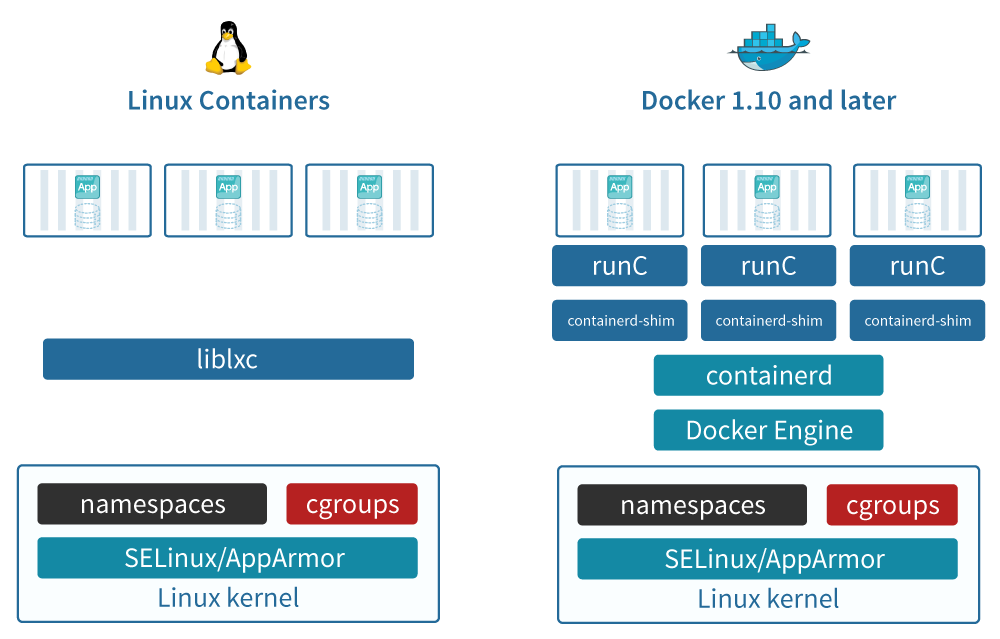
\includegraphics[width=5.20833in,height=3.33333in]{assets/lxc-vs-docker.png}\\

Jak widać na powyższej ilustracji zarówno \passthrough{\lstinline!LXC!}
jak i \passthrough{\lstinline!Docker!} bazują na kernelu
\passthrough{\lstinline!Linuxa!}, w tym:
\passthrough{\lstinline!SELinux!} lub
\passthrough{\lstinline!AppArmor!}, namespaces i
\passthrough{\lstinline!cGroups!}. Różnią się natomiast implementacją
samych kontenerów - \passthrough{\lstinline!LXC!} korzysta jedynie z
\passthrough{\lstinline!liblxc!}, a \passthrough{\lstinline!Docker!}
postanowił zaimplementować~wielopoziomowy system:
\passthrough{\lstinline!Docker Engine!},
\passthrough{\lstinline!containerd!} i \passthrough{\lstinline!runc!}.

\hypertarget{cel-pracy-inux17cynierskiej}{%
\section{Cel pracy inżynierskiej}\label{cel-pracy-inux17cynierskiej}}

Celem tej pracy jest: 1) przedstawienie podstawowych pojęć związanych z
aktualnie najpopularniejszym rozwiązaniem zarządzania kontenerami o
nazwie \passthrough{\lstinline!k8s!}, 2) przegląd dostępnych rozwiązań
oraz wdrożenie tego systemu w sieci uczelnianej na potrzeby prowadzenia
laboratoriów ze studentami.

Wdrożenie w sieci uczelnianej wiąże się z koniecznością uruchomienia
systemu z sieci na maszynach bezdyskowych.

Celem dodatkowym jest przeprowadzenie testów wydajnościowych klastra
\passthrough{\lstinline!k8s!}.

\hypertarget{przeglux105d-pojux119ux107-i-systemuxf3w-zwiux105zanych-z-konteneryzacjux105}{%
\chapter{Przegląd pojęć i systemów związanych z
konteneryzacją}\label{przeglux105d-pojux119ux107-i-systemuxf3w-zwiux105zanych-z-konteneryzacjux105}}

Wiodącym, ale nie jedynym, rozwiązaniem konteneryzacji jest
\passthrough{\lstinline!Docker!}.

\hypertarget{open-container-initiative}{%
\section{Open Container Initiative}\label{open-container-initiative}}

\href{https://www.opencontainers.org/about}{\passthrough{\lstinline!Open Container Initiative!}}
jest inicjatywą tworzenia i utrzymywania publicznych standardów
związanych z tworzeniem i obsługą kontenerów.

Większość projektów związanych z konteneryzacją dąży do kompatybilności
ze standardami \passthrough{\lstinline!OCI!}, m. in.:

\begin{itemize}
\tightlist
\item
  \href{https://blog.docker.com/2017/07/demystifying-open-container-initiative-oci-specifications/}{\passthrough{\lstinline!Docker!}}
\item
  \href{https://github.com/kubernetes-incubator/cri-o}{\passthrough{\lstinline!Kubernetes CRI-O!}}
\item
  \href{https://wiki.freebsd.org/Docker}{\passthrough{\lstinline!Docker on FreeBSD!}}
\item
  \href{https://www.youtube.com/watch?v=akLa9L5O0NY}{\passthrough{\lstinline!Running CloudABI applications on a FreeBSD based Kubernetes cluster, by Ed Schouten (EuroBSDcon '17)!}}
\end{itemize}

\hypertarget{docker}{%
\section{Docker}\label{docker}}

\passthrough{\lstinline!Docker!} jest najstarszym i w związku z tym
aktualnie najpopularniejszym rozwiązaniem problemu konteneryzacji.

Dobrym przeglądem alternatyw dla \passthrough{\lstinline!Dockera!} jest
\href{https://coreos.com/rkt/docs/latest/rkt-vs-other-projects.html}{porównianie
\passthrough{\lstinline!rkt!} z innymi rozwiązaniami} na oficjalnej
stronie \passthrough{\lstinline!CoreOS!}.

Domyślnie obrazy są pobierane przez internet z
\href{https://hub.docker.com/}{\passthrough{\lstinline!Docker Huba!}},
co jest ograniczone przepustowością łącza. Na wolne łącze możemy
zaradzić kieszeniując zapytania HTTP ub uruchamiając
\href{https://docs.docker.com/registry/deploying/}{rejestr obrazów} w
sieci lokalnej. Lokalny rejestr może być ograniczony do obrazów ręcznie
w nim umieszczonych lub udostępniać i kieszeniować~obrazy z zewnętrznego
rejestru (np. \passthrough{\lstinline!Docker Hub!}). Pierwsze
rozwiązanie w połączeniu z zablokowaniem dostępu do zewnętrznych
rejestrów daje prawie pełną kontrolę nad obrazami uruchamianymi wewnątrz
sieci.

\hypertarget{dostux119pne-rozwiux105zania-zarzux105dzania-kontenerami}{%
\section{Dostępne rozwiązania zarządzania
kontenerami}\label{dostux119pne-rozwiux105zania-zarzux105dzania-kontenerami}}

\hypertarget{kubernetes}{%
\subsubsection{Kubernetes}\label{kubernetes}}

\href{https://kubernetes.io/}{Kubernetes} (dalej jako
\passthrough{\lstinline!k8s!}) jest obecnie najpopularniejszym
narzędziem orkiestracji kontenerami, a przez to tematem przewodnim tego
dokumentu.

Został stworzony przez \passthrough{\lstinline!Google!} na bazie ich
wewnętrznego systemu Borg.

W porównaniu do innych narzędzi \passthrough{\lstinline!k8s!} oferuje
najlepszy kompromis między oferowanymi możliwościami, a kosztem
zarządzania.

Dobrym przeglądem alternatyw \passthrough{\lstinline!k8s!} jest artykuł
pt.
\href{https://dzone.com/articles/choosing-the-right-containerization-and-cluster-management-tool}{\passthrough{\lstinline!Choosing the Right Containerization and Cluster Management Tool!}}.

\hypertarget{fleet}{%
\subsubsection{Fleet}\label{fleet}}

\href{https://github.com/coreos/fleet}{\passthrough{\lstinline!Fleet!}}
jest nakładką~na
\href{https://www.freedesktop.org/wiki/Software/systemd/}{\passthrough{\lstinline!systemd!}}
realizująca rozproszony system inicjalizacji systemów w systemie
operacyjnym \passthrough{\lstinline!CoreOS!}.

Kontenery są~uruchamiane i zarządzane przez
\passthrough{\lstinline!systemd!}, a stan przechowywany jest w etcd.

Aktualnie projekt kończy swój żywot na rzecz
\passthrough{\lstinline!k8s!} i w dniu 1 lutego 2018, został wycofany z
domyślnej dystrybucji \passthrough{\lstinline!CoreOS!}. Nadal będzie
dostępny w rejestrze pakietów \passthrough{\lstinline!CoreOS!}.

\hypertarget{docker-swarm}{%
\subsubsection{Docker Swarm}\label{docker-swarm}}

\href{https://docs.docker.com/engine/swarm/}{\passthrough{\lstinline!Docker Swarm!}}
jest rozwiązaniem orkiestracji kontenerami od twórców samego
\passthrough{\lstinline!Dockera!}. Proste w obsłudze, ale nie oferuje
tak dużych możliwości jak inne rozwiązania.

\hypertarget{nomad}{%
\subsubsection{Nomad}\label{nomad}}

\href{https://www.nomadproject.io/intro/index.html}{\passthrough{\lstinline!Nomad!}}
od \passthrough{\lstinline!HashiCorp!} jest narzędziem do zarządzania
klastrem, które również oferuje zarządzanie kontenerami.

Przy jego tworzeniu twórcy kierują się filozofią
\passthrough{\lstinline!Unix!}. W związku z tym Nomad jest prosty w
obsłudze, wyspecjalizowany i rozszerzalny. Zwykle działa w tandemie z
innymi produktami HashiCorp jak Consul i Vault.

Porównanie z innymi rozwiązaniami możemy znaleźć na oficjalnej stronie
\passthrough{\lstinline!Nomada!}:
\href{https://www.nomadproject.io/intro/vs/index.html}{\passthrough{\lstinline!HashiCorp Nomad vs Other Software!}}

\hypertarget{mesos}{%
\subsubsection{Mesos}\label{mesos}}

\href{http://mesos.apache.org/}{\passthrough{\lstinline!Apache Mesos!}}
jest najbardziej zaawansowanym i najlepiej skalującym się rozwiązaniem
orkiestracji kontenerami. Jest również najbardziej skomplikowanym i
trudnym w zarządzaniu rozwiązaniem, w związku z tym znajduje swoje
zastosowanie tylko w największych systemach komputerowych.

Dobrym wstępem do zagadnienia jest ten artykuł:
\href{https://www.digitalocean.com/community/tutorials/an-introduction-to-mesosphere}{\passthrough{\lstinline!An Introduction to Mesosphere!}}.

\hypertarget{kubernetes-1}{%
\chapter{Kubernetes}\label{kubernetes-1}}

W tym rozdziale opiszę zagadnienia związane z samym systemem
\passthrough{\lstinline!k8s!}.

\hypertarget{administracja-a-korzystanie-z-klastra}{%
\section{Administracja, a korzystanie z
klastra}\label{administracja-a-korzystanie-z-klastra}}

Przez zwrot \passthrough{\lstinline!administracja klastrem!} (lub
zarządzanie nim) rozumiem zbiór czynności i procesów polegających na
przygotowaniu klastra do użytku i zarządzanie jego infrastrukturą. Na
przykład: tworzenie klastra, dodawanie i usuwanie węzłów oraz nadawanie
uprawnień innym użytkownikom.

Przez zwrot \passthrough{\lstinline!korzystanie z klastra!} rozumiem
uruchamianie aplikacji na działającym klastrze.

Ze względu na ograniczone zasoby czasu w tej pracy inżynierskiej skupiam
się na kwestiach związanych z administracją klastrem.

\hypertarget{konfiguracja-klastra}{%
\section{Konfiguracja klastra}\label{konfiguracja-klastra}}

Ważną~kwestią jest zrozumienie pojęcia stanu w klastrze
\passthrough{\lstinline!k8s!}. Jest to stan do którego klaster dąży, a
nie w jakim się w danej chwili znajduje.

Zwykle stan docelowy i aktywny szybko się ze sobą~zbiegają, ale nie jest
to regułą. Najczęstszymi scenariuszami jest brak zasobów do uruchomienia
aplikacji w klastrze lub zniknięcie węzła roboczego.

W pierwszym przypadku stan klastra może wskazywać na istnienie 5
instancji aplikacji, ale pamięci RAM wystarcza na uruchomienie tylko 3.
Więc bez zmiany infrastruktury brakujące 2 instancje nigdy nie zostaną
uruchomione. W momencie dołączenia kolejnego węzła klastra może się
okazać, że posiadamy już oczekiwane zasoby i aplikacja zostanie
uruchomiona w pełni.

W drugim przypadku załóżmy, że aplikacja jest uruchomiona w 9 kopiach na
4 węzłach, po 2 kopię na pierwszych trzech węzłach i 3 kopie na
ostatnim. W momencie wyłączenia ostatniego węzła aplikacja będzie miała
uruchomione tylko 6 z 9 docelowych instancji. Zanim moduł kontrolujący
klaster zauważy braki aktywny stan 6 nie będzie się zgadzał z docelowym
9. W ciągu kilku do kilkudziesięciu sekund kontroler uruchomi brakujące
3 instancje i uzyskamy docelowy stan klastra: po 3 kopie aplikacji na 3
węzłach.

\hypertarget{infrastruktura-kubernetesa}{%
\section{Infrastruktura Kubernetesa}\label{infrastruktura-kubernetesa}}

Infrastrukturę definiuję jako część~odpowiadającą za funkcjonowanie
klastra, a nie za aplikacje na nim działające. Z infrastrukturą wiążę
pojęcie administracji klastrem.

Zdecydowałem się przybliżyć temat na podstawie
\href{https://commons.wikimedia.org/wiki/File:Kubernetes.png}{jednego
diagramu znalezionego na wikimedia.org}:

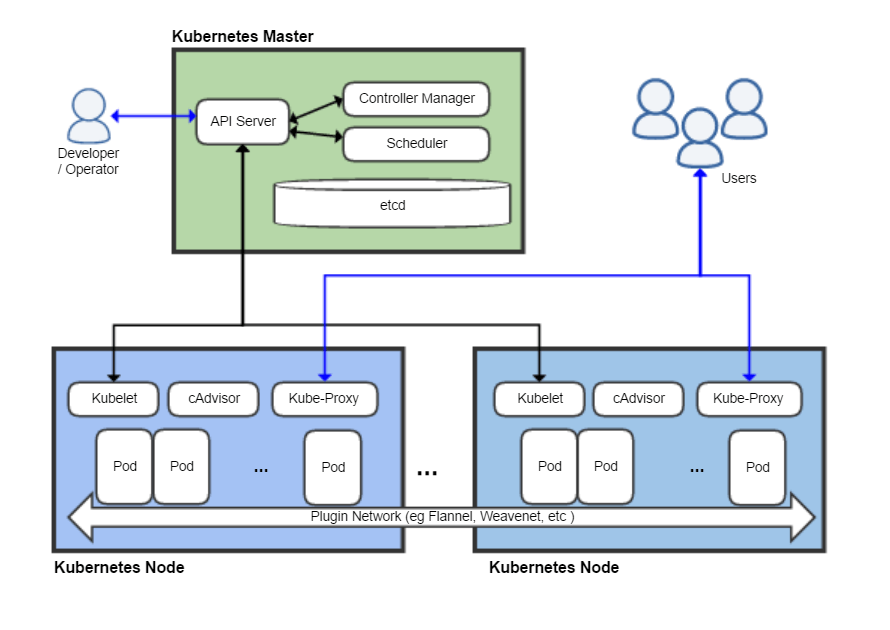
\includegraphics[width=5.20833in,height=3.6875in]{assets/kubernetes-architecture.png}\\

Na ilustracji możemy wyróżnić 5 grup funkcjonalnych:

\begin{enumerate}
\def\labelenumi{\arabic{enumi}.}
\tightlist
\item
  \passthrough{\lstinline!Developer/Operator!}, czyli administrator lub
  programista korzystający z klastra,
\item
  \passthrough{\lstinline!Users!}, czyli użytkowników aplikacji
  działających w klastrze,
\item
  \passthrough{\lstinline!Kubernetes Master!}, czyli węzeł zarządzający
  (zwykle więcej niż~jeden),
\item
  \passthrough{\lstinline!Kubernetes Node!}, czyli jeden z wielu węzłów
  roboczych, na których działają aplikacje,
\item
  \passthrough{\lstinline!Plugin Network!}, czyli wtyczka sieciowa
  realizująca lub konfigurująca połączenia pomiędzy kontenerami
  działającymi w ramach klastra,
\end{enumerate}

\hypertarget{wux119zeux142-zarzux105dzajux105cy}{%
\subsubsection{Węzeł
zarządzający}\label{wux119zeux142-zarzux105dzajux105cy}}

Stan \passthrough{\lstinline!k8s!} jest przechowywany w
\href{https://coreos.com/etcd/}{\passthrough{\lstinline!etcd!}}. Nazwa
wzięła się od Unixowego folderu \passthrough{\lstinline!/etc!}
przechowującego konfigurację systemu operacyjnego i litery
\passthrough{\lstinline!d!} oznaczającej system rozproszony (ang.
distributed system). Jest to baza danych przechowująca jedynie klucze i
wartości (ang. key-value store). Koncepcyjnie jest prosta, żeby
umożliwić skupienie się na jej wydajności, stabilności i skalowaniu.

Jedynym sposobem zmiany stanu \passthrough{\lstinline!etcd!}
(zakładając, że nie jest wykorzystywane do innych celów) jest
komunikacja z
\href{https://kubernetes.io/docs/reference/generated/kube-apiserver/}{\passthrough{\lstinline!kube-apiserver!}}.
Zarówno zewnętrzni użytkownicy jak i wewnętrzne procesy klastra
korzystają z interfejsu aplikacyjnego REST (ang. REST API) klastra w
celu uzyskania informacji i zmiany jego stanu.

Głównym modułem zarządzającym, który dba o doprowadzenia klastra do
oczekiwanego stanu jest
\href{https://kubernetes.io/docs/reference/generated/kube-controller-manager/}{\passthrough{\lstinline!kube-controller-manager!}}.
Uruchamia on pętle kontrolujące klaster, na której bazuje wiele procesów
kontrolnych jak na przykład kontroler replikacji i kontroler kont
serwisowych.

Modułem zarządzającym zasobami klastra jest
\href{https://kubernetes.io/docs/reference/generated/kube-scheduler/}{\passthrough{\lstinline!kube-scheduler!}}.
Decyduje on na których węzłach uruchamiać aplikacje, żeby zaspokoić
popyt na zasoby jednocześnie nie przeciążając pojedynczych węzłów
klastra.

\hypertarget{wux119zeux142-roboczy}{%
\subsubsection{Węzeł roboczy}\label{wux119zeux142-roboczy}}

Podstawowym procesem działającym na węzłach roboczych jest
\href{https://kubernetes.io/docs/reference/generated/kubelet/}{\passthrough{\lstinline!kubelet!}}.
Monitoruje i kontroluje kontenery działające w ramach jednego węzła. Na
przykład wiedząc, że na węźle mają działać 2 instancje aplikacji dba o
to, żeby restartować instancje działające nieprawidłowo~i/lub
dodawać~nowe.

Drugim najważniejszym procesem węzła roboczego jest
\passthrough{\lstinline!kube-proxy!} odpowiadające za przekierowywanie
ruchu sieciowego do odpowiednich kontenerów w ramach klastra.

Ostatnim opcjonalnym elementem węzła roboczego jest
\href{https://github.com/google/cadvisor}{\passthrough{\lstinline!cAdvisor!}}
(Container Advisor), który monitoruje zużycie zasobów i wydajność
kontenerów w ramach jednego klastra.

\hypertarget{wtyczka-sieciowa}{%
\subsubsection{Wtyczka sieciowa}\label{wtyczka-sieciowa}}

Podstawowym założeniem \passthrough{\lstinline!k8s!} jest posiadanie
własnego adresu IP przez każdą aplikację działającą w klastrze, ale nie
narzuca żadnego rozwiązania je realizującego.

Administrator (lub skrypt konfigurujący) klastra musi zadbać o to, żeby
skonfigurować wtyczkę sieciową realizującą to założenie.

Najprostszym koncepcyjnie rozwiązaniem jest stworzenie na każdym węźle
wpisów \passthrough{\lstinline!iptables!} przekierowujących adresy IP na
wszystkie inne węzły.

Jednymi z najpopularniejszymi rozwiązaniami są:
\href{https://github.com/coreos/flannel\#flannel}{Flannel} i
\href{https://www.projectcalico.org/}{Project Calico}.

\hypertarget{komunikacja-sieciowa}{%
\subsubsection{Komunikacja sieciowa}\label{komunikacja-sieciowa}}

Materiały źródłowe:

\begin{itemize}
\tightlist
\item
  https://www.slideshare.net/weaveworks/kubernetes-networking-78049891
\item
  https://jvns.ca/blog/2016/12/22/container-networking/
\item
  https://medium.com/@anne\_e\_currie/kubernetes-aws-networking-for-dummies-like-me-b6dedeeb95f3
\end{itemize}

4 rodzaje komunikacji sieciowej:

\begin{enumerate}
\def\labelenumi{\arabic{enumi}.}
\tightlist
\item
  wewnątrz Podów (localhost)
\item
  między Podami (trasowanie lub nakładka sieciowa - overlay network)
\item
  między Podami i Serwisami (kube-proxy)
\item
  świata z Serwisami
\end{enumerate}

W skrócie:

\begin{itemize}
\tightlist
\item
  \passthrough{\lstinline!k8s!} uruchamia
  \passthrough{\lstinline!Pody!}, które implementują~Serwisy,
\item
  \passthrough{\lstinline!Pody!}
  potrzebują~\passthrough{\lstinline!Sieci Pod!}ów - trasowanych lub
  nakładkę sieciową,
\item
  Sieć \passthrough{\lstinline!Pod!}ów jest sterowana przez
  \passthrough{\lstinline!CNI!} (Container Network Interface),
\item
  Klient łączy się~do Serwisów przez wirtualne IP Klastra,
\item
  \passthrough{\lstinline!k8s!} ma wiele sposobów na wystawienie
  Serwisów poza klaster,
\end{itemize}

\hypertarget{zarzux105dzanie-dostux119pami}{%
\subsubsection{Zarządzanie
dostępami}\label{zarzux105dzanie-dostux119pami}}

Podstawowymi pojęciami związanymi z zarządzaniem dostępami w
\passthrough{\lstinline!k8s!} są uwierzytelnianie, autoryzacja i
\passthrough{\lstinline!Namespace!}.

\hypertarget{uwierzytelnianie}{%
\paragraph{Uwierzytelnianie}\label{uwierzytelnianie}}

Pierwszym krokiem w każdym zapytaniu do API jest uwierzytelnienie, czyli
weryfikacja, że użytkownik (czy to aplikacja) jest tym za kogo się
podaje. Podstawowymi sposobami uwierzytelniania są:

\begin{itemize}
\tightlist
\item
  certyfikaty klienckie X509,
\item
  statyczne przepustki (ang. \passthrough{\lstinline!token!}),
\item
  przepustki rozruchowe (ang.
  \passthrough{\lstinline!bootstrap tokens!}),
\item
  statyczny plik z hasłami,
\item
  przepustki kont serwisowych (ang.
  \passthrough{\lstinline!ServiceAccount!} tokens),
\item
  przepustki OpenID Connect,
\item
  Webhook (zapytanie uwierzytelniające do zewnętrznego serwisu),
\item
  proxy uwierzytelniające,
\end{itemize}

Ze względu na prostotę i uniwersalność~rozwiązania w tej pracy będę
korzystał z \passthrough{\lstinline!ServiceAccount!}.

\hypertarget{autoryzacja}{%
\paragraph{Autoryzacja}\label{autoryzacja}}

Drugim krokiem jest autoryzacja, czyli weryfikacja, że użytkownik jest
uprawniony do korzystania z danego zasobu.

Najpopularniejszym sposobem autoryzacji jest
\href{https://kubernetes.io/docs/admin/authorization/rbac/}{RBAC (Role
Based Access Control)}. Odbywa się ona na podstawie ról
(\passthrough{\lstinline!Role!} i
\passthrough{\lstinline!ClusterRole!}), które nadają uprawnienia i są
przypisywane konkretnym użytkownikom lub kontom przez
\passthrough{\lstinline!RoleBinding!} i
\passthrough{\lstinline!ClusterRoleBinding!}.

\passthrough{\lstinline!Namespace!} (przestrzeń nazw) jest logicznie
odseparowaną częścią~klastra \passthrough{\lstinline!k8s!}. Pozwala na
współdzielenie jednego klastra przez wielu niezaufanych użytkowników.
Standardowym zastosowaniem jest wydzielanie środowisk produkcyjnych, QA
i deweloperskich.

Jak nazwa wskazuje role z dopiskiem \passthrough{\lstinline!Cluster!}
mogą dać dostęp do wszystkich przestrzeni nazw jednocześnie oraz zasobów
takowych nie posiadających. Przykładem zasobu nie posiadającego swojej
przestrzeni nazw jest węzeł (\passthrough{\lstinline!Node!}) lub
zakończenie API \passthrough{\lstinline!/healthz!}.

Role bez dopisku \passthrough{\lstinline!Cluster!} operują w ramach
jednej przestrzeni nazw.

\hypertarget{architektura}{%
\section{Architektura}\label{architektura}}

Architekturę klastra definiuję jako część aplikacyjną, czyli wszystkie
funkcjonalności dostępne po przeprowadzeniu prawidłowej konfiguracji
klastra i oddaniu węzłów do użytku. Z architekturą wiążę pojęcia
korzystania z klastra, stanu i obiektów \passthrough{\lstinline!k8s!}.

\hypertarget{obiekty-kubernetes-api}{%
\subsubsection{Obiekty Kubernetes API}\label{obiekty-kubernetes-api}}

\href{https://kubernetes.io/docs/concepts/overview/working-with-objects/kubernetes-objects/}{\passthrough{\lstinline!Obiekty Kubernetesa!}}
są trwale przechowywane w \passthrough{\lstinline!etcd!} i definiują,
jak wcześniej wyjaśniłem, pożądany stan klastra. Szczegółowy opis
konwencji API obiektów możemy znaleźć~w
\href{https://github.com/kubernetes/community/blob/master/contributors/devel/api-conventions.md}{odnośniku}.

Jako użytkownicy klastra operujemy na ich reprezentacji w formacie YAML,
a rzadziej JSON, na przykład:

\begin{lstlisting}
apiVersion: v1
kind: Pod
metadata:
  name: my-pod 
  namespace: my-namespace
  uid: 343fc305-c854-44d0-9085-baed8965e0a9
  labels:
    resources: high
  annotations:
    app-type: qwe
spec:
  containers:
  - image: ubuntu:trusty
    command: ["echo"]
    args: ["Hello World"]
  ...
status:
  podIP: 127.12.13.14
  ...
\end{lstlisting}

W każdym obiekcie możemy wyróżnić~trzy obowiązkowe i dwa opcjonalne
pola:

\begin{itemize}
\tightlist
\item
  \passthrough{\lstinline!apiVersion!}: obowiązkowa wersja API
  \passthrough{\lstinline!k8s!},
\item
  \passthrough{\lstinline!kind!}: obowiązkowy typ obiektu zdefiniowanego
  w specyfikacji \passthrough{\lstinline!apiVersion!},
\item
  \passthrough{\lstinline!metadata!}

  \begin{itemize}
  \tightlist
  \item
    \passthrough{\lstinline!namespace!}: opcjonalna (domyślna
    \passthrough{\lstinline!default!}) przestrzeń nazw do której należy
    obiekt,
  \item
    \passthrough{\lstinline!name!}: obowiązkowa i unikalna w ramach
    przestrzeni nazw nazwa obiektu,
  \item
    \passthrough{\lstinline!uid!}: unikalny identyfikator obiektu tylko
    do odczytu,
  \item
    \passthrough{\lstinline!labels!}: opcjonalny zbiór kluczy i wartości
    ułatwiających identyfikację i grupowanie obiektów,
  \item
    \passthrough{\lstinline!annotations!}: opcjonalny zbiór kluczy i
    wartości wykorzystywanych przez zewnętrzne lub własne narzędzia,\\
  \end{itemize}
\item
  \passthrough{\lstinline!spec!}: z definicji opcjonalna, ale zwykle
  wymagana specyfikacja obiektu wpływająca na jego funkcjonowanie,
\item
  \passthrough{\lstinline!status!}: opcjonalny aktualny stan obiektu
  tylko do odczytu,
\end{itemize}

\hypertarget{podstawowe-rodzaje-obiektuxf3w-aplikacyjnych}{%
\subsubsection{Podstawowe rodzaje obiektów
aplikacyjnych}\label{podstawowe-rodzaje-obiektuxf3w-aplikacyjnych}}

Ważną kwestią jest rozróżnienie obiektów imperatywnych i deklaratywnych.
Obiekty imperatywne reprezentują wykonanie akcji, a deklaratywne
określają stan w jakim klaster powinien się znaleźć.

\hypertarget{pod}{%
\paragraph{Pod`}\label{pod}}

\href{https://kubernetes.io/docs/concepts/workloads/pods/pod-overview/}{\passthrough{\lstinline!Pod!}}
jest najmniejszą jednostką aplikacyjną~w \passthrough{\lstinline!k8s!}.
Reprezentuje nierozłącznie powiązaną~(np. współdzielonymi zasobami)
grupę jednego lub więcej kontenerów.

\passthrough{\lstinline!Pod!} w odróżnieniu od innych obiektów
reprezentuje aktualnie działającą aplikację. Są bezustannie uruchamiane
i wyłączane przez kontrolery. Trwałość danych można uzyskać
jedynie~przydzielając im zasoby dyskowe.

\passthrough{\lstinline!Pody!} nie powinny być zarządzane bezpośrednio,
jedynie przez kontrolery. Najczęściej konfigurowane są przez
\passthrough{\lstinline!PodTemplateSpec!}, czyli szablony ich
specyfikacji.

Kontenery wewnątrz \passthrough{\lstinline!Poda!} współdzielą~adres IP i
mogą komunikować się przez \passthrough{\lstinline!localhost!} i
standardowe metody komunikacji międzyprocesowej.

Dodatkowo kontenery wewnątrz \passthrough{\lstinline!Pod!}ów obsługują 2
rodzaje
\href{https://kubernetes.io/docs/concepts/workloads/pods/pod-lifecycle/\#container-probes}{próbników}:
\passthrough{\lstinline!livenessProbe!} i
\passthrough{\lstinline!readinessProbe!}. Pierwszy określa, czy kontener
działa, jeżeli nie to powinien być zrestartowany. Drugi określa czy
kontener jest gotowy do obsługi zapytań, kontener jest wyrejestrowywany
z \passthrough{\lstinline!Service!} na czas nieprzechodzenia
\passthrough{\lstinline!readinessProbe!}.

\hypertarget{replicaset}{%
\paragraph{ReplicaSet`}\label{replicaset}}

\href{https://kubernetes.io/docs/concepts/workloads/controllers/replicaset/}{\passthrough{\lstinline!ReplicaSet!}}
jest następcą \passthrough{\lstinline!ReplicaControllera!}, czyli
imperatywnym kontrolerem dbającym o działanie określonej liczby
\passthrough{\lstinline!Pod!}ów w klastrze.

Jest to bardzo prosty kontroler i nie powinien być~używany bezpośrednio.

\hypertarget{deployment}{%
\paragraph{Deployment`}\label{deployment}}

\href{https://kubernetes.io/docs/concepts/workloads/controllers/deployment/}{\passthrough{\lstinline!Deployment!}}
pozwala na deklaratywne aktualizacje \passthrough{\lstinline!Pod!}ów i
\passthrough{\lstinline!ReplicaSet!}ów. Korzystanie z ww. bezpośrednio
nie jest zalecane.

Zmiany \passthrough{\lstinline!Deployment!}ów wprowadzane są przez tak
zwane \passthrough{\lstinline!rollouty!}. Każdy ma swój status i może
zostać wstrzymany lub przerwany. \passthrough{\lstinline!Rollouty!} mogą
zostać aktywowane automatycznie przez zmianę specyfikacji
\passthrough{\lstinline!Pod!}a przez
\passthrough{\lstinline!.spec.template!}.

Rewizje \passthrough{\lstinline!Deployment!}u są zmieniane tylko w
momencie \passthrough{\lstinline!rollout!}u. Operacja operacja
skalowania nie uruchamia \passthrough{\lstinline!rollout!}u, a więc nie
zmienia rewizji.

Podstawowe przypadki użycia \passthrough{\lstinline!Deployment!} to:

\begin{itemize}
\tightlist
\item
  uruchamianie \passthrough{\lstinline!ReplicaSet!}ów w tle przez
  \passthrough{\lstinline!.spec.replicas!},
\item
  deklarowanie nowego stanu \passthrough{\lstinline!Pod!}ów zmieniając
  \passthrough{\lstinline!.spec.template!},
\item
  cofanie zmian do poprzednich rewizji
  \passthrough{\lstinline!Deployment!}u (poprzednie wersje
  \passthrough{\lstinline!Pod!}ów) komendą
  \passthrough{\lstinline!kubectl rollout undo!},
\item
  skalowanie \passthrough{\lstinline!Deployment!}u w celu obsługi
  większego obciążenia przykładową komendą
  \passthrough{\lstinline!kubectl autoscale deployment nginx-deployment --min=10 --max=15 --cpu-percent=80!},
\item
  wstrzymywanie \passthrough{\lstinline!Deployment!} w celu wprowadzenia
  poprawek komendą
  \passthrough{\lstinline!kubectl rollout pause deployment/nginx-deployment!},
\item
  czyszczenie historii \passthrough{\lstinline!ReplicaSet!}ów przez
  ograniczanie liczby wpisów w
  \passthrough{\lstinline!.spec.revisionHistoryLimit!},
\end{itemize}

Przykładowy \passthrough{\lstinline!Deployment!} tworzący 3 repliki
serwera \passthrough{\lstinline!nginx!}:

\begin{lstlisting}
apiVersion: apps/v1
kind: Deployment
metadata:
  name: nginx-deployment
  labels:
    app: nginx
spec:
  replicas: 3
  selector:
    matchLabels:
      app: nginx
  template:
    metadata:
      labels:
        app: nginx
    spec:
      containers:
      - name: nginx
        image: nginx:1.7.9
        ports:
        - containerPort: 80
\end{lstlisting}

Pole \passthrough{\lstinline!.spec.selector!} definiuje w jaki sposób
\passthrough{\lstinline!Deployment!} ma znaleźć
\passthrough{\lstinline!Pod!}y, którymi ma zarządzać. Selektor powinien
zgadzać się ze zdefiniowanym szablonem.

\hypertarget{statefulset}{%
\paragraph{StatefulSet}\label{statefulset}}

\href{https://kubernetes.io/docs/concepts/workloads/controllers/statefulset/}{\passthrough{\lstinline!StatefulSet!}}
jest kontrolerem podobnym do \passthrough{\lstinline!Deployment!}u, ale
umożliwiającym zachowanie stanu \passthrough{\lstinline!Pod!}ów.

W przeciwieństwie do \passthrough{\lstinline!Deployment!}
\passthrough{\lstinline!StatefulSet!} nadaje każdemu uruchomionemu
\passthrough{\lstinline!Pod!}owi stały unikalny identyfikator, który
zostają zachowane mimo restartów i przenoszenia
\passthrough{\lstinline!Pod!}ów. Identyfikatory można zastosować między
innymi do:

\begin{itemize}
\tightlist
\item
  trwałych i unikalnych identyfikatorów wewnątrz sieci,
\item
  trwałych zasobów dyskowych,
\item
  sekwencyjne uruchamianie i skalowanie aplikacji,
\item
  sekwencyjne zakańczanie i usuwanie aplikacji,
\item
  sekwencyjne, zautomatyzowane aktualizacje aplikacji,
\end{itemize}

\hypertarget{daemonset}{%
\paragraph{DaemonSet}\label{daemonset}}

\href{https://kubernetes.io/docs/concepts/workloads/controllers/daemonset/}{\passthrough{\lstinline!DaemonSet!}}
jest kontrolerem upewniającym się, że przynajmniej jeden
\passthrough{\lstinline!Pod!} działa na każdym lub wybranych węzłach
klastra.

Do jego typowych zastosowań należy implementacja narzędzi wymagających
agenta na każdym z węzłów:

\begin{itemize}
\tightlist
\item
  rozproszone systemy dyskowe, np. \passthrough{\lstinline!glusterd!},
  \passthrough{\lstinline!ceph!},
\item
  zbieracze logów, np. \passthrough{\lstinline!fluentd!},
  \passthrough{\lstinline!logstash!},
\item
  monitorowanie węzłów, np.
  \passthrough{\lstinline!Prometheus Node Exporter!},
  \passthrough{\lstinline!collectd!},
\end{itemize}

\hypertarget{job-i-cronjob}{%
\paragraph{Job i CronJob}\label{job-i-cronjob}}

\href{https://kubernetes.io/docs/concepts/workloads/controllers/jobs-run-to-completion/}{\passthrough{\lstinline!Job!}}
pozwala na jednorazowe uruchomienie \passthrough{\lstinline!Pod!}ów,
które wykonują akcję i się kończą. Istnieją~3 tryby wykonania:
niezrównoleglony, równoległy i równoległy z zewnętrzną kolejką zadań.

Domyślnie przy niepowodzeniu uruchamiane są~kolejne
\passthrough{\lstinline!Pody!} aż~zostanie uzyskana odpowiednia liczba
sukcesów.

\href{https://kubernetes.io/docs/concepts/workloads/controllers/cron-jobs/}{\passthrough{\lstinline!CronJob!}}
pozwala na tworzenie \passthrough{\lstinline!Job!}ów jednorazowo o
określonym czasie lub je powtarzać zgodnie ze
specyfikacją~\href{https://en.wikipedia.org/wiki/Cron}{\passthrough{\lstinline!cron!}}.

\hypertarget{kubernetes-dashboard}{%
\section{Kubernetes Dashboard}\label{kubernetes-dashboard}}

\href{https://github.com/kubernetes/dashboard}{\passthrough{\lstinline!Kubernetes Dashboard!}}
jest wbudowanym interfejsem graficznym klastra
\passthrough{\lstinline!k8s!}. Umożliwia monitorowanie i zarządzanie
klastrem w ramach funkcjonalności samego \passthrough{\lstinline!k8s!}.

\hypertarget{kubernetes-incubator}{%
\section{Kubernetes Incubator}\label{kubernetes-incubator}}

\href{https://github.com/kubernetes/community/blob/master/incubator.md}{\passthrough{\lstinline!Kubernetes Incubator!}}
gromadzi projekty rozszerzające \passthrough{\lstinline!k8s!}, ale nie
będące częścią oficjalnej dystrybucji. Został stworzony, aby opanować
bałagan w głównym repozytorium oraz ujednolicić proces tworzenia
rozszerzeń.

Aby dołączyć do inkubatora projekt musi spełnić szereg wymagań oraz nie
może spędzić w inkubatorze więcej niż 18 miesięcy. Dostępne opcje
opuszczenia inkubatora to:

\begin{itemize}
\tightlist
\item
  awansować do rangi oficjalnego projektu \passthrough{\lstinline!k8s!},
\item
  połączyć się z istniejącym oficjalnym projektem,
\item
  po 12 miesiącach przejść w stan spoczynku, a po kolejnych 6 miesiącach
  zostać przeniesiony do
  \passthrough{\lstinline!kubernetes-incubator-retired!}
\end{itemize}

\hypertarget{administracja-klastrem-z-linii-komend}{%
\section{Administracja klastrem z linii
komend}\label{administracja-klastrem-z-linii-komend}}

\hypertarget{kubeadm}{%
\subsubsection{kubeadm}\label{kubeadm}}

\href{https://kubernetes.io/docs/reference/setup-tools/kubeadm/kubeadm/}{kubeadm}
jest narzędziem pozwalającym na niskopoziomowe zarządzanie klastrem
\passthrough{\lstinline!k8s!}. Stąd trendem jest bazowanie na kubeadm
przy tworzeniu narzędzi z wyższym poziomem abstrakcji.

\begin{itemize}
\tightlist
\item
  \href{https://kubernetes.io/docs/setup/independent/install-kubeadm/}{Install
  with kubadm}
\end{itemize}

\hypertarget{kubespray}{%
\subsubsection{Kubespray}\label{kubespray}}

\href{https://github.com/kubernetes-incubator/kubespray}{kubespray} jest
zbiorem skryptów Ansibla konfigurujących klaster na różnych systemach
operacyjnych i w różnych konfiguracjach. W tym jest w stanie
skonfigurować klaster bare metal bez żadnych zewnętrznych zależności.

Projekt na dzień dzisiejszy znajduje się w inkubatorze i jest aktywnie
rozwijany.

\hypertarget{openshift-ansible}{%
\subsubsection{OpenShift Ansible}\label{openshift-ansible}}

Konfiguracja \protect\hyperlink{openshift-origin}{OpenShift Origin}
realizowana jest zestawem skryptów Ansible'owych rozwijanych jako
projekt
\href{https://github.com/openshift/openshift-ansible}{openshift-ansible}.

\hypertarget{canonical-distribution-of-kubernetes}{%
\subsubsection{Canonical distribution of
Kubernetes}\label{canonical-distribution-of-kubernetes}}

Jest to prosta w instalacji dystrybucja \passthrough{\lstinline!k8s!}.
Niestety wymaga infrastruktury chmurowej do uruchomienia klastra
składającego się z więcej niż jednego węzła.

Opcja \passthrough{\lstinline!bare metal!}, która by mnie interesowała
nadal wymaga działającego środowiska \href{https://maas.io/}{Metal as a
Service}.

W związku z powyższym nie będę dalej zajmował się tym narzędziem.

Materiały źródłowe:

\begin{itemize}
\tightlist
\item
  \href{https://jujucharms.com/canonical-kubernetes/}{pakiet
  (\passthrough{\lstinline!Charm!}) w oficjalnym repozytorium
  \passthrough{\lstinline!Juju!}}
\item
  \href{https://tutorials.ubuntu.com/tutorial/install-kubernetes-with-conjure-up}{materiał
  szkoleniowy dot. uruchamiania \passthrough{\lstinline!k8s!}}
\item
  \href{https://insights.ubuntu.com/2017/10/12/kubernetes-the-not-so-easy-way/}{opis
  instalacji lokalnego klastra}
\end{itemize}

\hypertarget{bootkube-i-typhoon}{%
\subsubsection{Bootkube i Typhoon}\label{bootkube-i-typhoon}}

\href{https://github.com/kubernetes-incubator/bootkube}{\passthrough{\lstinline!Bootkube!}}
jest narzędziem napisanym w języku \passthrough{\lstinline!Go!}
pozwalającym skonfigurować \passthrough{\lstinline!k8s!} na własnych
maszynach.

W instalacji
\href{https://github.com/coreos/matchbox/tree/master/examples/terraform/bootkube-install}{\passthrough{\lstinline!bare metal!}}
proponowane jest wykorzystanie \passthrough{\lstinline!Terraform!} i
\href{https://github.com/poseidon/typhoon}{\passthrough{\lstinline!Typhoon!}}
do realizacji automatycznej konfiguracji klastra w trakcie procesu
uruchamiania węzłów \passthrough{\lstinline!CoreOS!}.

Domyślnie ww. narzędzia konfigurują instalację CoreOS na dysku, a
następnie restartują maszynę.

W wyniku przeoczenia wzmianki (przypis na jednej z podstron
dokumentacji) o możliwości uruchomienia w trybie bezdyskowym całkowicie
odrzuciłem to narzędzie. W końcowych etapach pisania pracy znalazłem ww.
wpis i zdecydowałem się zawrzeć o nim informację.

\hypertarget{eksperymentalne-i-deprekowane-rozwiux105zania}{%
\subsubsection{Eksperymentalne i deprekowane
rozwiązania}\label{eksperymentalne-i-deprekowane-rozwiux105zania}}

\begin{itemize}
\tightlist
\item
  \href{https://kubernetes.io/docs/getting-started-guides/fedora/fedora_ansible_config/}{\passthrough{\lstinline!Fedora via Ansible!}}
  deprekowane na rzecz \passthrough{\lstinline!kubespray!}
\item
  \href{http://rancher.com/announcing-rke-lightweight-kubernetes-installer/}{\passthrough{\lstinline!Rancher Kubernetes Installer!}}
  jest eksperymentalnym rozwiązaniem wykorzystywanym w Rancher 2.0,
\end{itemize}

\hypertarget{kubespray-cli}{%
\paragraph{kubespray-cli}\label{kubespray-cli}}

Jest to narzędzie ułatwiające korzystanie z
\passthrough{\lstinline!kubespray!}. Według użytkowników
\href{https://kubernetes.slack.com/messages/kubespray}{oficjalnego
\passthrough{\lstinline!Slacka!} \passthrough{\lstinline!kubespray!}}
\passthrough{\lstinline!kubespray-cli!} jest deprekowane i powinno
się~korzystać~z czystego \passthrough{\lstinline!kubespray!}.

\hypertarget{administracja-klastrem-za-pomocux105-narzux119dzi-graficznych}{%
\section{Administracja klastrem za pomocą narzędzi
graficznych}\label{administracja-klastrem-za-pomocux105-narzux119dzi-graficznych}}

\hypertarget{rancher}{%
\subsubsection{Rancher}\label{rancher}}

\href{https://rancher.com/}{Rancher} jest platformą~zarządzania
kontenerami umożliwiającą między innymi zarządzanie klastrem
\passthrough{\lstinline!k8s!}. Od wersji 2.0 twórcy skupiają się
wyłącznie na zarządzaniu \passthrough{\lstinline!k8s!} porzucając
wsparcie innych rozwiązań.

\hypertarget{openshift-origin}{%
\subsubsection{OpenShift by Red Hat}\label{openshift-origin}}

OpenShift jest komercyjną~usługą typu \passthrough{\lstinline!PaaS!}
(Platform as a Service), od wersji 3 skupia się na zarządzaniu klastrem
\passthrough{\lstinline!k8s!}.

Rdzeniem projektu jest open sourcowy
\href{https://github.com/openshift/origin}{OpenShift Origin}
konfigurowany przez \protect\hyperlink{openshift-ansible}{OpenShift
Ansible}.

Materiały źródłowe:

\begin{itemize}
\tightlist
\item
  \href{https://www.reddit.com/r/devops/comments/59ql4r/openshift_origin_vs_kubernetes/}{dyskusja
  o wykorzystaniu \passthrough{\lstinline!OpenShift Origin!} i
  \passthrough{\lstinline!k8s!}}
\item
  \href{https://medium.com/levvel-consulting/the-differences-between-kubernetes-and-openshift-ae778059a90e}{opis
  różnic między \passthrough{\lstinline!OpenShift Origin!} i
  \passthrough{\lstinline!k8s!}}
\item
  \href{https://youtu.be/-mFovK19aB4?t=6m54s}{materiał wideo
  przedstawiający interfejs OpenShift} (po hebrajsku)
\end{itemize}

\hypertarget{dcos}{%
\subsubsection{DC/OS}\label{dcos}}

\href{https://dcos.io/}{Datacenter Operating System} jest częścią
\href{https://mesosphere.com/}{Mesosphere} i Mesosa. Niedawno został
rozszerzony o
\href{https://mesosphere.com/blog/kubernetes-dcos/}{\passthrough{\lstinline!k8s!}}
jako alternatywny (w stosunku do
\href{https://mesosphere.github.io/marathon/}{\passthrough{\lstinline!Marathon!}})
system orkiestracji kontenerami.

\hypertarget{lista-materiaux142uxf3w-dodatkowych}{%
\section{Lista materiałów
dodatkowych}\label{lista-materiaux142uxf3w-dodatkowych}}

Ze względu na obszerność tematu zdecydowałem przedstawić oddzielną listę
materiałów dodatkowych:

\begin{itemize}
\tightlist
\item
  \href{https://jvns.ca/categories/kubernetes/}{blog Julii Evans o
  \passthrough{\lstinline!k8s!}},
\item
  \href{https://github.com/kelseyhightower/kubernetes-the-hard-way}{dokument
  o uruchamianiu \passthrough{\lstinline!k8s!} od podstaw},
\item
  \href{https://www.youtube.com/watch?v=4-pawkiazEg}{materiał wideo o
  skalowaniu \passthrough{\lstinline!k8s!}},
\end{itemize}

\hypertarget{systemy-bezdyskowe}{%
\chapter{Systemy bezdyskowe}\label{systemy-bezdyskowe}}

Maszyny bezdyskowe jak nazwa wskazuje nie posiadają lokalnego medium
trwałego przechowywania informacji. W związku z tym wszystkie informacje
są przechowywane w pamięci RAM komputera i są tracone w momencie
restartu maszyny.

System operacyjny musi wspierać uruchamianie w takim środowisku. Wiele
systemów nie wspiera tego trybu operacyjnego zakładając obecność dysku
twardego w maszynie.

W niektórych przypadkach mimo braku domyślnego wsparcia istnieje
możliwość przygotowania własnego obrazu systemu operacyjnego
wspierającego ten tryb pracy:

\begin{itemize}
\tightlist
\item
  \href{https://www.projectatomic.io/blog/2015/05/building-and-running-live-atomic/}{Fedora
  Atomic Host}.
\end{itemize}

Potencjalnymi rozwiązaniami problemu przechowywania stanu maszyn
bezdyskowych mogą być:

\begin{itemize}
\tightlist
\item
  przydziały NFS,
\item
  \href{https://arstechnica.com/information-technology/2015/12/rsync-net-zfs-replication-to-the-cloud-is-finally-here-and-its-fast/}{replikacja
  ZFS},
\item
  przechowywanie całego stanu w
  \protect\hyperlink{cloud-init-config}{cloud-init}.
\end{itemize}

\hypertarget{proces-uruchamiania-maszyny-bezdyskowej}{%
\section{Proces uruchamiania maszyny
bezdyskowej}\label{proces-uruchamiania-maszyny-bezdyskowej}}

Na uruchamianie maszyn bezdyskowych w protokole PXE składają się 3
podstawowe elementy:

\begin{enumerate}
\def\labelenumi{\arabic{enumi}.}
\tightlist
\item
  serwer DHCP, np. isc-dhcp-server lub dnsmasq,
\item
  firmware wspierające PXE, np. iPXE,
\item
  serwer plików (np. TFTP, HTTP, NFS) i/lub sieciowej pamięci masowej
  (np. iSCSI).
\end{enumerate}

Pełną lokalną~konfigurację bazowaną na Dockerze przechowuję w moim
repozytorium \href{https://github.com/nazarewk/ipxe-boot}{ipxe-boot}.

\hypertarget{przeglux105d-systemuxf3w-operacyjnych}{%
\chapter{Przegląd systemów
operacyjnych}\label{przeglux105d-systemuxf3w-operacyjnych}}

Wszystkie moduły \passthrough{\lstinline!k8s!} są uruchamiane w
kontenerach, więc dwoma podstawowymi wymaganiami systemu operacyjnego
są:

\begin{itemize}
\tightlist
\item
  możliwość instalacji i uruchomienia Dockera,
\item
  wsparcie wybranego narzędzia konfigurującego system do działania w
  klastrze \passthrough{\lstinline!k8s!},
\end{itemize}

Dodatkowe wymagania związane z opisywanym w tej pracy przypadkiem
użycia:

\begin{itemize}
\tightlist
\item
  zdalny dostęp SSH lub możliwość konfiguracji automatycznego dołączania
  do klastra \passthrough{\lstinline!k8s!},
\item
  wsparcie dla środowiska bezdyskowego,
\item
  możliwość~bootu PXE.
\end{itemize}

Podstawowe wyznaczniki:

\begin{itemize}
\tightlist
\item
  sposób konfiguracji maszyny,
\item
  rozmiar minimalnego działającego systemu spełniającego wszystkie
  wymagania,
\item
  aktualne wersje oprogramowania.
\end{itemize}

\hypertarget{cloud-init-config}{%
\section{Konfigurator cloud-init}\label{cloud-init-config}}

Ze względu na obszerność~i niejednoznaczność tematu cloud-init
zdecydowałem się wyjaśnić wszelkie wątpliwości z nim związane.

\href{https://cloud-init.io/}{cloud-init} jest standardem oraz
implementacją konfiguratora kompatybilnego z wieloma systemami
operacyjnymi przeznaczonymi do działania w chmurze.

Standard polega na dostarczeniu pliku konfiguracyjnego w formacie
\href{http://yaml.org/}{YAML} w trakcie lub tuż po inicjalizacji systemu
operacyjnego.

Główną zaletą cloud-init jest tworzenie automatycznej i jednorodnej
konfiguracji bazowych systemów operacyjnych w środowiskach chmurowych,
czyli częstego podnoszenia nowych maszyn.

\hypertarget{dostux119pne-implementacje}{%
\subsubsection{Dostępne
implementacje}\label{dostux119pne-implementacje}}

\hypertarget{cloud-init}{%
\paragraph{cloud-init}\label{cloud-init}}

Referencyjny \passthrough{\lstinline!cloud-init!} zaimplementowany jest
w Pythonie, co częściowo tłumaczy duży rozmiar obrazów przeznaczonych
dla chmury. Po najmniejszych obrazach
\href{https://hub.docker.com/_/python/}{\passthrough{\lstinline!Pythona!}
dla \passthrough{\lstinline!Dockera!}} (python:alpine - 89MB i
python2:alpine - 72 MB) wnioskuję, że nie istnieje mniejsza dystrybucja
Pythona.

\begin{lstlisting}[language=bash]
docker pull python:2-alpine > /dev/null
docker pull python:alpine > /dev/null
docker images | grep alpine
\end{lstlisting}

Dodatkowe materiały:

\begin{itemize}
\tightlist
\item
  \href{https://www.podcastinit.com/cloud-init-with-scott-moser-episode-126}{Wywiad
  z developerem cloud-init}
\end{itemize}

\hypertarget{coreos-cloudinit}{%
\paragraph{coreos-cloudinit}\label{coreos-cloudinit}}

\href{https://github.com/coreos/coreos-cloudinit}{\passthrough{\lstinline!coreos-cloudinit!}}
jest częściową implementacją~standardu w języku Go udostępnioną przez
twórców \protect\hyperlink{coreos}{\passthrough{\lstinline!CoreOS!}}
\href{https://github.com/coreos/coreos-cloudinit/commit/3460ca4414fd91de66cd581d997bf453fd895b67}{Rok
temu przestał być~rozwijany} i wychodzi z użytku.

\hypertarget{rancheros-coreos-cloudinit}{%
\paragraph{RancherOS +
coreos-cloudinit}\label{rancheros-coreos-cloudinit}}

\href{http://rancher.com/docs/os/latest/en/configuration/}{\passthrough{\lstinline!Rancher cloud-init!}}
jest jest
\href{https://github.com/rancher/os/commit/e2ed97648ad63455743ebc16080a82ee47f8bb0c}{przejętym}
\protect\hyperlink{coreos-cloudinit}{\passthrough{\lstinline!coreos-cloudinit!}}
przez zespół
\protect\hyperlink{rancheros}{\passthrough{\lstinline!RancherOS!}}.

\hypertarget{clr-cloud-init}{%
\paragraph{clr-cloud-init}\label{clr-cloud-init}}

\href{https://clearlinux.org/blogs/announcing-clr-cloud-init}{\passthrough{\lstinline!clr-cloud-init!}}
jest wewnętrzną~implementacją~standardu dla systemu
\protect\hyperlink{clearlinux}{\passthrough{\lstinline!ClearLinux!}}.
Powstała z chęci optymalizacji standardu pod
\passthrough{\lstinline!ClearLinux!} oraz pozbycia się zależności
referencyjnej implementacji od \passthrough{\lstinline!Pythona!}.

\hypertarget{coreos}{%
\section{CoreOS}\label{coreos}}

\href{https://coreos.com/}{\passthrough{\lstinline!CoreOS!}} jest
pierwszą dystrybucją \passthrough{\lstinline!Linuxa!} przeznaczoną do
zarządzania kontenerami. Zawiera dużo narzędzi dedykowanych klastrowaniu
i obsłudze kontenerów, w związku z tym zajmuje 342 MB.

Czysta instalacja zajmuje około 600 MB pamięci RAM i posiada najnowsze
wersje Dockera i OverlayFS.

30 stycznia 2018 roku
\href{https://www.redhat.com/en/about/press-releases/red-hat-acquire-coreos-expanding-its-kubernetes-and-containers-leadership}{został
wykupiony przez Red Hat}.

\hypertarget{konfiguracja}{%
\subsubsection{Konfiguracja}\label{konfiguracja}}

Konfiguracja obsługiwana jest przez
\href{https://coreos.com/os/docs/latest/provisioning.html}{Container
Linux Config} transpilowany do
\href{https://coreos.com/ignition/docs/latest/}{Ignition}. Transpiler
konwertuje ogólną konfigurację na przygotowaną~pod konkretne chmury
(AWS, GCE, Azure itp.). Minusem jest brak dystrybucji transpilatora pod
\passthrough{\lstinline!FreeBSD!}.

Poprzednikiem~Ignition jest
\protect\hyperlink{coreos-cloudinit}{coreos-cloudinit}.

\hypertarget{rancheros}{%
\section{RancherOS}\label{rancheros}}

\href{https://rancher.com/rancher-os/}{RancherOS} jest systemem
operacyjnym, w którym tradycyjny system inicjalizacji został~zastąpiony
\href{http://rancher.com/docs/os/latest/en/configuration/docker/}{trzema
poziomami Dockera}:

\begin{itemize}
\tightlist
\item
  \passthrough{\lstinline!bootstrap\_docker!} - działający w initramie,
  czyli przygotowuje system,
\item
  \passthrough{\lstinline!system-docker!} - zastępuje tradycyjny init,
  zarządza wszystkimi programami systemowymi,
\item
  \passthrough{\lstinline!docker!} - standardowy
  \passthrough{\lstinline!Docker!}, interakcja z nim nie może uszkodzić
  działającego systemu.
\end{itemize}

Jego głównymi zaletami są mały rozmiar plików startowych (45 MB) oraz
prostota konfiguracji.

Czysta instalacja zajmuje około 700 MB pamięci RAM. Niestety nie jest
często aktualizowany i posiada stare wersje zarówno Dockera (17.06
sprzed pół roku) jak i \passthrough{\lstinline!overlay!} (zamiast
\passthrough{\lstinline!overlay2!}).

W związku z bugiem w systemie RancherOS
\href{https://github.com/rancher/os/issues/2204}{nie zawsze czyta
cloud-config}, więc odrzucam ten system operacyjny w dalszych
rozważaniach.

\hypertarget{ros-config}{%
\subsubsection{Konfiguracja}\label{ros-config}}

\passthrough{\lstinline!RancherOS!} jest konfigurowany przez
\protect\hyperlink{rancheros-+-coreos-cloudinit}{własną~wersję}
coreos-cloudinit.

Znaczną przewagą wobec oryginału jest możliwość~sekwencyjnego
uruchamiania dowolnej liczby plików konfiguracyjnych.

Minimalna konfiguracja pozwalająca na zalogowanie:

\begin{lstlisting}
#cloud-config
ssh_authorized_keys:
  - ssh-rsa <klucz RSA>
\end{lstlisting}

Generuję ją poniższym skryptem na podstawie komendy
\passthrough{\lstinline!ssh-add -L!}:

\begin{lstlisting}[language=bash]
#!/bin/sh

cat << EOF > ssh.yml
#cloud-config
ssh_authorized_keys:
$(ssh-add -L | sed 's/^/  - /g')
EOF
\end{lstlisting}

Przydatne jest wyświetlenie kompletnej konfiguracji komendą
\href{https://forums.rancher.com/t/good-cloud-config-reference/5238/3}{\passthrough{\lstinline!ros config export --full!}}.

\hypertarget{project-atomic}{%
\section{Project Atomic}\label{project-atomic}}

\href{https://www.projectatomic.io/}{\passthrough{\lstinline!Project Atomic!}}
jest grupą~podobnie skonfigurowanych systemów operacyjnych dedykowaną
środowiskom cloud i kontenerom.

Dystrybucje \passthrough{\lstinline!Project Atomic!} nazywają~się
\passthrough{\lstinline!Atomic Host!}. Dostępne są ich następujące
warianty:

\begin{itemize}
\tightlist
\item
  \href{https://www.redhat.com/en/resources/enterprise-linux-atomic-host-datasheet}{Red
  Hat Atomic Host},
\item
  \href{https://wiki.centos.org/SpecialInterestGroup/Atomic/Download/}{CentOS
  Atomic Host},
\item
  \href{https://getfedora.org/atomic/download/}{Fedora Atomic Host}.
\end{itemize}

Żadna z dystrybucji domyślnie nie wspiera rozruchu bezdyskowego, więc
nie zgłębiam dalej tematu.

\passthrough{\lstinline!Atomic Host!} są konfigurowane oficjalną
implementacją~\passthrough{\lstinline!cloud-inita!}.

\hypertarget{alpine-linux}{%
\section{Alpine Linux}\label{alpine-linux}}

\href{https://alpinelinux.org/}{Alpine Linux} jest minimalną dystrybucją
Linuxa bazowaną na musl-libc i busybox.

Wygląda bardzo obiecująco w kontekście moich zastosowań, ale ze względu
na buga w procesie inicjalizacji systemu aktualnie nie ma możliwości
jego uruchomienia w trybie bezdyskowym.

Alpine Linux może być~skonfigurowany przez
\href{https://wiki.alpinelinux.org/wiki/Alpine_local_backup}{Alpine
Backup} lub
\href{http://wiki.alpinelinux.org/wiki/Alpine_Configuration_Framework_Design}{Alpine
Configuration Framework}.

\hypertarget{clearlinux}{%
\section{ClearLinux}\label{clearlinux}}

\href{https://clearlinux.org/}{ClearLinux} jest dystrybucją
\passthrough{\lstinline!Linuxa!} wysoko zoptymalizowaną pod procesory
Intel.

Poza intensywną optymalizacją ciekawy w tej dystrybucji jest koncept
\passthrough{\lstinline!bundle!} zamiast standardowych pakietów
systemowych. Żaden z bundli nie może zostać zaktualizowany oddzielnie, w
zamian cały system operacyjny jest aktualizowany na raz ze wszystkimi
bundlami. Znacznie ułatwia to zarządzanie wersjami oprogramowania i
stanem poszczególnych węzłów sieci komputerowej.

Czysta instalacja z Dockerem i serwerem SSH również zajmuje 700 MB
pamięci RAM więc nie odbiega od innych dystrybucji.

Ogromnym minusem jest trudna w nawigowaniu dokumentacja systemu
operacyjnego.

Materiały źródłowe:

\begin{itemize}
\tightlist
\item
  \href{https://www.infoworld.com/article/3159658/linux/6-key-points-about-intels-hot-new-linux-distro.html}{6
  key points about Intel's hot new Linux distro}
\end{itemize}

\hypertarget{wnioski}{%
\section{Wnioski}\label{wnioski}}

Głównymi czynnikami odróżniającymi poszczególne systemy operacyjne są
częstotliwość aktualizacji oprogramowania oraz wsparcie narzędzi.
Rozbieżność reszty parametrów jest pomijalnie mała.

Najczęściej aktualizowanym z powyższych systemów jest CoreOS, więc na
nim skupię się w dalszej części pracy.

\hypertarget{praktyczne-rozeznanie-w-narzux119dziach-administracji-klastrem-kubernetesa}{%
\chapter{Praktyczne rozeznanie w narzędziach administracji klastrem
Kubernetesa}\label{praktyczne-rozeznanie-w-narzux119dziach-administracji-klastrem-kubernetesa}}

Najpopularniejszym rozwiązaniem konfiguracji klastra
\passthrough{\lstinline!k8s!} jest
\href{https://github.com/kubernetes/kops}{\passthrough{\lstinline!kops!}},
ale jak większość rozwiązań zakłada uruchomienie w środowiskach
chmurowych, \passthrough{\lstinline!PaaS!} lub
\passthrough{\lstinline!IaaS!}. W związku z tym nie ma żadnego
zastosowania w tej pracy inżynierskiej.

\hypertarget{kubespray-cli-1}{%
\section{kubespray-cli}\label{kubespray-cli-1}}

Z powodu
\href{https://github.com/kubespray/kubespray-cli/issues/120}{błędu}
logiki narzędzie nie radzi sobie z brakiem
\passthrough{\lstinline!Pythona!} na domyślnej dystrybucji
\passthrough{\lstinline!CoreOSa!}, mimo że sam
\passthrough{\lstinline!kubespray!} radzi sobie z nim świetnie.

Do uruchomienia na tym systemie potrzebne jest ręczne wywołanie roli
\href{https://github.com/kubernetes-incubator/kubespray/blob/master/roles/bootstrap-os/tasks/main.yml}{\passthrough{\lstinline!bootstrap-os!}}
z \passthrough{\lstinline!kubespray!} zanim przystąpi się do właściwego
deployment'u. Skrypt uruchamiający:

\begin{lstlisting}[language=bash]
#!/bin/sh
set -e

# pip2 install ansible kubespray
get_coreos_nodes() {
  for node in $@
  do
    echo -n node1[
    echo -n ansible_host=${node},
    echo -n bootstrap_os=coreos,
    echo -n ansible_user=core,
    echo -n ansible_default_ipv4.address=${node}
    echo ]
  done
}

NODES=($(get_coreos_nodes 192.168.56.{10,12,13}))
echo NODES=${NODES[@]}
kubespray prepare -y --nodes ${NODES[@]}

cat << EOF > ~/.kubespray/bootstrap-os.yml
- hosts: all
  become: yes
  gather_facts: False
  roles:
  - bootstrap-os
EOF

(
  cd ~/.kubespray;
  ansible-playbook -i inventory/inventory.cfg bootstrap-os.yml
)
kubespray deploy -y --coreos
\end{lstlisting}

\hypertarget{napotkane-problemy}{%
\subsubsection{Napotkane problemy}\label{napotkane-problemy}}

Narzędzie kończy się błędem na kroku czekania na uruchomienie
\passthrough{\lstinline!etcd!}, ponieważ oczekuje połączenia na NATowym
interfejsie z adresem \passthrough{\lstinline!10.0.3.15!} zamiast host
network z adresem \passthrough{\lstinline!192.168.56.10!}, stąd ręczne
podawanie \passthrough{\lstinline!ansible\_default\_ipv4.address!}.

\hypertarget{wnioski-1}{%
\subsubsection{Wnioski}\label{wnioski-1}}

W trakcie testowania okazało się, że
\passthrough{\lstinline!kubespray-cli!} nie jest aktywnie rozwiązane i
stało się niekompatybilne z samym projektem
\passthrough{\lstinline!Kubespray!}. W związku z tym uznaję
\passthrough{\lstinline!kubespray-cli!} za nie mające zastosowania w tej
pracy inżynierskiej.

\hypertarget{rancher-kubernetes}{%
\section{Rancher 2.0}\label{rancher-kubernetes}}

Jest to wygodne narzędzie do uruchamiania i monitorowania klastra
\passthrough{\lstinline!k8s!}, ale wymaga interakcji użytkownika. Wersja
2.0 (obecnie w fazie alpha) oferuje lepszą integrację z
\passthrough{\lstinline!k8s!} całkowicie porzucając inne platformy.

W trakcie pisania pracy (24 stycznia 2018) pojawiło się drugie Tech
Preview. W stosunku do pierwszego Tech Preview aplikacja została mocno
przebudowana i nie wspiera jeszcze konfiguracji
\passthrough{\lstinline!bare metal!}, więc jestem zmuszony odrzucić to
rozwiązanie.

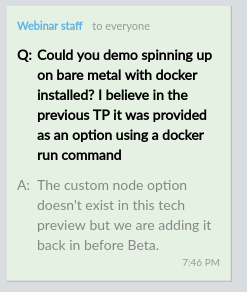
\includegraphics{assets/rancher-tp2-baremetal.png}\\

\hypertarget{testowanie-tech-preview-1-v2.0.0-alpha10}{%
\subsubsection{Testowanie tech preview 1
(v2.0.0-alpha10)}\label{testowanie-tech-preview-1-v2.0.0-alpha10}}

\begin{lstlisting}[language=bash]
#rancher_version=latest
#rancher_version=preview
rancher_version=v2.0.0-alpha10
docker run --rm --name rancher -d -p 8080:8080 rancher/server:${rancher_version}
\end{lstlisting}

Najpierw należy zalogować się~do panelu administracyjnego Ranchera i
przeprowadzić podstawową konfigurację (adres Ranchera + uzyskanie
komendy).

Następnie w celu dodania węzła do klastra wystarczy wywołać jedną
komendę~ udostępnioną w panelu administracyjnym Ranchera na docelowym
węźle, jej domyślny format to:

\begin{lstlisting}[language=bash]
wersja_agenta=v1.2.9
ip_ranchera=192.168.56.1
skrypt=B52944BEFAA613F0CE90:1514678400000:E2yB6KfxzSix4YHti39BTw5RbKw

sudo docker run --rm --privileged \
  -v /var/run/docker.sock:/var/run/docker.sock \
  -v /var/lib/rancher:/var/lib/rancher \
  rancher/agent:${wersja_agenta} \
  http://${ip_ranchera}:8080/v1/scripts/${skrypt}
\end{lstlisting}

W ciągu 2 godzin przeglądu nie udało mi się zautomatyzować procesu
uzyskiwania ww. komendy.

Następnie w \passthrough{\lstinline!cloud-configu!}
\passthrough{\lstinline!RancherOSa!} możemy dodać ww. komendę w formie:

\begin{lstlisting}
#cloud-config
runcmd:
- docker run --rm --privileged -v /var/run/docker.sock:/var/run/docker.sock -v /var/lib/rancher:/var/lib/rancher rancher/agent:v1.2.9 http://192.168.56.1:8080/v1/scripts/...
\end{lstlisting}

Od wersji 2.0 umożliwia połączenie się z istniejącym klastrem:

\begin{lstlisting}
kubectl apply -f http://192.168.56.1:8080/v3/scripts/303F60E1A5E186F53F3F:1514678400000:wstQFdHpOgHqKahoYdmsCXEWMW4.yaml
\end{lstlisting}

\hypertarget{napotkane-bux142ux119dy}{%
\paragraph{Napotkane błędy}\label{napotkane-bux142ux119dy}}

W wersji \passthrough{\lstinline!v2.0.0-alpha10!} losowo pojawia
się~błąd \href{https://github.com/rancher/rancher/issues/10396}{Upgrade
Environment}.

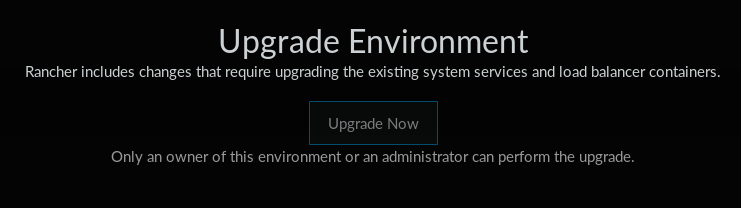
\includegraphics[width=5.20833in,height=1.45833in]{assets/rancher2-error.png}\\

\hypertarget{wnioski-2}{%
\subsubsection{Wnioski}\label{wnioski-2}}

Rancher na chwilę obecną (styczeń 2018 roku) jest bardzo wygodnym, ale
również niestabilnym rozwiązaniem.

Ze względu na brak stabilności odrzucam Ranchera jako rozwiązanie
problemu uruchamiania klastra \passthrough{\lstinline!k8s!}.

\hypertarget{openshift-origin-1}{%
\section{OpenShift Origin}\label{openshift-origin-1}}

Według
\href{https://docs.openshift.org/latest/getting_started/administrators.html}{dokumentacji}
są~dwie metody uruchamiania serwera, w
\passthrough{\lstinline!Dockerze!} i bezpośrednio na systemie
\passthrough{\lstinline!Linux!}.

\begin{lstlisting}[language=bash]
# https://docs.openshift.org/latest/getting_started/administrators.html#installation-methods
docker run -d --name "origin" \
  --privileged --pid=host --net=host \
  -v /:/rootfs:ro \
  -v /var/run:/var/run:rw \
  -v /sys:/sys \
  -v /sys/fs/cgroup:/sys/fs/cgroup:rw \
  -v /var/lib/docker:/var/lib/docker:rw \
  -v /var/lib/origin/openshift.local.volumes:/var/lib/origin/openshift.local.volumes:rslave \
  openshift/origin start --public-master
\end{lstlisting}

Dodałem opcję \passthrough{\lstinline!--public-master!} aby uruchomić
konsolę webową

\hypertarget{korzystanie-ze-sterownika-systemd-zamiast-domyux15blnego-cgroupfs}{%
\subsubsection{Korzystanie ze sterownika systemd zamiast domyślnego
cgroupfs}\label{korzystanie-ze-sterownika-systemd-zamiast-domyux15blnego-cgroupfs}}

Większość dystrybucji \passthrough{\lstinline!Linuxa!} (np. Arch,
CoreOS, Fedora, Debian) domyślnie nie konfiguruje sterownika cgroup
Dockera i korzysta z domyślnego \passthrough{\lstinline!cgroupfs!}.

Typ sterownika cgroup można wyświetlić komendą
\passthrough{\lstinline!docker info!}:

\begin{lstlisting}
$ docker info | grep -i cgroup
Cgroup Driver: systemd
\end{lstlisting}

OpenShift natomiast konfiguruje \passthrough{\lstinline!k8s!} do
korzystania z \passthrough{\lstinline!cgroup!} przez
\passthrough{\lstinline!systemd!}. Kubelet przy starcie weryfikuje
zgodność silników cgroup, co
\href{https://github.com/openshift/origin/issues/14766}{skutkuje
niekompatybilnością z domyślną konfiguracją Dockera}, czyli poniższym
błędem:

\begin{lstlisting}
F0120 19:18:58.708005   25376 node.go:269] failed to run Kubelet: failed to create kubelet: misconfiguration: kubelet cgroup driver: "systemd" is different from docker cgroup driver: "cgroupfs"
\end{lstlisting}

Problem można rozwiązać dopisując
\passthrough{\lstinline!--exec-opt native.cgroupdriver=systemd!} do
linii komend \passthrough{\lstinline!dockerd!} (zwykle w pliku
\passthrough{\lstinline!docker.service!}). Dla przykładu w
\passthrough{\lstinline!Arch Linuksie!} zmiana wygląda następująco:

\begin{lstlisting}
$ cp /usr/lib/systemd/system/docker.service /etc/systemd/system/docker.service
$ vim /etc/systemd/system/docker.service
$ diff /usr/lib/systemd/system/docker.service /etc/systemd/system/docker.service
13c13
< ExecStart=/usr/bin/dockerd -H fd://
---
> ExecStart=/usr/bin/dockerd -H fd:// --exec-opt native.cgroupdriver=systemd
\end{lstlisting}

\hypertarget{pruxf3ba-uruchomienia-serwera-na-arch-linux}{%
\subsubsection{Próba uruchomienia serwera na Arch
Linux}\label{pruxf3ba-uruchomienia-serwera-na-arch-linux}}

Po wystartowaniu serwera zgodnie z dokumentacją~OpenShift Origin i
naprawieniu błędu z konfiguracją~cgroup przeszedłem do kolejnego kroku
\href{https://docs.openshift.org/latest/getting_started/administrators.html\#try-it-out}{Try
It Out}:

\begin{enumerate}
\def\labelenumi{\arabic{enumi}.}
\tightlist
\item
  Uruchomienie shella na serwerze:
\end{enumerate}

\begin{lstlisting}
$ docker exec -it origin bash
\end{lstlisting}

\begin{enumerate}
\def\labelenumi{\arabic{enumi}.}
\setcounter{enumi}{1}
\tightlist
\item
  Logowanie jako testowy użytkownik:
\end{enumerate}

\begin{lstlisting}
$ oc login
Username: test
Password: test
\end{lstlisting}

\begin{enumerate}
\def\labelenumi{\arabic{enumi}.}
\setcounter{enumi}{2}
\tightlist
\item
  Stworzenie nowego projektu:
\end{enumerate}

\begin{lstlisting}
$ oc new-project test
\end{lstlisting}

\begin{enumerate}
\def\labelenumi{\arabic{enumi}.}
\setcounter{enumi}{3}
\tightlist
\item
  Pobranie aplikacji z Docker Huba:
\end{enumerate}

\begin{lstlisting}
$ oc tag --source=docker openshift/deployment-example:v1 deployment-example:latest
\end{lstlisting}

\begin{enumerate}
\def\labelenumi{\arabic{enumi}.}
\setcounter{enumi}{4}
\tightlist
\item
  Wystartowanie aplikacji:
\end{enumerate}

\begin{lstlisting}
$ oc new-app deployment-example:latest
\end{lstlisting}

\begin{enumerate}
\def\labelenumi{\arabic{enumi}.}
\setcounter{enumi}{5}
\tightlist
\item
  Odczekanie aż~aplikacja się uruchomi:
\end{enumerate}

\begin{lstlisting}
$ watch -n 5 oc status
In project test on server https://192.168.0.87:8443

svc/deployment-example - 172.30.52.184:8080
  dc/deployment-example deploys istag/deployment-example:latest 
    deployment #1 failed 1 minute ago: config change
\end{lstlisting}

Niestety nie udało się przejść kroku 5, więc próba uruchomienia
OpenShift Origin na Arch Linux zakończyła się niepowodzeniem.

\hypertarget{pruxf3ba-uruchomienia-serwera-na-fedora-atomic-host-w-virtualbox}{%
\subsubsection{Próba uruchomienia serwera na Fedora Atomic Host w
VirtualBox}\label{pruxf3ba-uruchomienia-serwera-na-fedora-atomic-host-w-virtualbox}}

Maszynę z najnowszym \passthrough{\lstinline!Fedora Atomic Host!}
uruchomiłem za pomocą poniższego \passthrough{\lstinline!Vagrantfile!}:

\begin{lstlisting}[language=Ruby]
# -*- mode: ruby -*-
# vi: set ft=ruby :

Vagrant.configure("2") do |config|
  config.vm.box = "fedora/27-atomic-host"
  config.vm.box_check_update = false
  config.vm.network "forwarded_port", guest: 8443, host: 18443, host_ip: "127.0.0.1"
  config.vm.network "forwarded_port", guest: 8080, host: 18080, host_ip: "127.0.0.1"
  config.vm.provider "virtualbox" do |vb|
    vb.gui = false
    vb.memory = "8192"
  end
  config.vm.provision "shell", inline: <<-SHELL
  SHELL
end
\end{lstlisting}

\begin{lstlisting}
$ vagrant up
$ vagrant ssh
$ sudo docker run -d --name "origin" \
  --privileged --pid=host --net=host \
  -v /:/rootfs:ro \
  -v /var/run:/var/run:rw \
  -v /sys:/sys \
  -v /sys/fs/cgroup:/sys/fs/cgroup:rw \
  -v /var/lib/docker:/var/lib/docker:rw \
  -v /var/lib/origin/openshift.local.volumes:/var/lib/origin/openshift.local.volumes:rslave \
  openshift/origin start
\end{lstlisting}

Kroki 1-5 były analogiczne do uruchamiania na
\passthrough{\lstinline!Arch Linux!}, następnie:

\begin{enumerate}
\def\labelenumi{\arabic{enumi}.}
\setcounter{enumi}{5}
\tightlist
\item
  Odczekanie aż~aplikacja się uruchomi i weryfikacja działania:
\end{enumerate}

\begin{lstlisting}
$ watch -n 5 oc status
In project test on server https://10.0.2.15:8443

svc/deployment-example - 172.30.221.105:8080
  dc/deployment-example deploys istag/deployment-example:latest 
    deployment #1 deployed 3 seconds ago - 1 pod
$ curl http://172.30.221.105:8080 | grep v1
<div class="box"><h1>v1</h1><h2></h2></div>
\end{lstlisting}

\begin{enumerate}
\def\labelenumi{\arabic{enumi}.}
\setcounter{enumi}{6}
\tightlist
\item
  Aktualizacja, przebudowanie i weryfikacja działania aplikacji:
\end{enumerate}

\begin{lstlisting}
$ oc tag --source=docker openshift/deployment-example:v2 deployment-example:latest
Tag deployment-example:latest set to openshift/deployment-example:v2.
$ watch -n 5 oc status
In project test on server https://10.0.2.15:8443

svc/deployment-example - 172.30.221.105:8080
  dc/deployment-example deploys istag/deployment-example:latest 
    deployment #2 running for 8 seconds - 1 pod
    deployment #1 deployed 8 minutes ago - 1 pod
$ curl -s http://172.30.221.105:8080 | grep v2
<div class="box"><h1>v2</h1><h2></h2></div>
\end{lstlisting}

\begin{enumerate}
\def\labelenumi{\arabic{enumi}.}
\setcounter{enumi}{7}
\tightlist
\item
  Nie udało się uzyskać dostępu do panelu administracyjnego OpenShift:
\end{enumerate}

\begin{lstlisting}
$ curl -k 'https://localhost:8443/console/'
missing service (service "webconsole" not found)
missing route (service "webconsole" not found)
\end{lstlisting}

W internecie nie znalazłem żadnych informacji na temat tego błędu.
Próbowałem również uzyskać pomoc na kanale
\passthrough{\lstinline!#openshift!} na
\passthrough{\lstinline!irc.freenode.net!}, ale bez skutku.

\hypertarget{wnioski-3}{%
\subsubsection{Wnioski}\label{wnioski-3}}

Panel administracyjny klastra \passthrough{\lstinline!OpenShift Origin!}
jest jedyną~znaczącą przewagą nad \passthrough{\lstinline!Kubesprayem!}.
Reszta zarządzania klastrem odbywa się również za pomocą repozytorium
skryptów Ansibla
(\href{https://docs.openshift.com/enterprise/3.0/admin_guide/manage_nodes.html\#adding-nodes}{w
tym dodawanie kolejnych węzłów klastra}).

Z powodu braku dostępu do ww. panelu próbę uruchomienia
\passthrough{\lstinline!OpenShift Origin!} uznaję za nieudaną i odrzucam
to narzędzie.

\hypertarget{kubespray-1}{%
\section{kubespray}\label{kubespray-1}}

Cały kod znajduje się w moim repozytorium
\href{https://github.com/nazarewk/kubernetes-cluster}{kubernetes-cluster}.

\hypertarget{kubernetes-dashboard-1}{%
\subsubsection{Kubernetes Dashboard}\label{kubernetes-dashboard-1}}

Dostęp do Dashboardu najprościej można uzyskać poprzez:

\begin{enumerate}
\def\labelenumi{\arabic{enumi}.}
\tightlist
\item
  \href{https://github.com/kubernetes/dashboard/wiki/Access-control\#admin-privileges}{nadanie
  wszystkich uprawnień roli
  \passthrough{\lstinline!kubernetes-dashboard!}},
\item
  Wejście pod adres
  \passthrough{\lstinline"http://localhost:8001/api/v1/namespaces/kube-system/services/https:kubernetes-dashboard:/proxy/#!/login"}
  ,
\item
  Kliknięcie skip.
\end{enumerate}

Materiały źródłowe:

\begin{itemize}
\tightlist
\item
  https://github.com/kubernetes/dashboard/wiki/Access-control
\item
  https://github.com/kubernetes-incubator/kubespray/blob/master/docs/getting-started.md\#accessing-kubernetes-dashboard
\end{itemize}

\hypertarget{napotkane-bux142ux119dy-1}{%
\subsubsection{Napotkane błędy}\label{napotkane-bux142ux119dy-1}}

Błąd przy ustawieniu
\passthrough{\lstinline!loadbalancer\_apiserver.address!} na
\passthrough{\lstinline!0.0.0.0!}:

\begin{lstlisting}
TASK [kubernetes-apps/cluster_roles : Apply workaround to allow all nodes with cert O=system:nodes to register] ****
Wednesday 17 January 2018  22:22:59 +0100 (0:00:00.626)       0:08:31.946 *****
fatal: [node2]: FAILED! => {"changed": false, "msg": "error running kubectl (/opt/bin/kubectl apply --force --filename=/etc/kubernetes/node-crb.yml) command (rc=1): Unable to connect to the server: http: server gave HTTP response to HTTPS client"}
fatal: [node1]: FAILED! => {"changed": false, "msg": "error running kubectl (/opt/bin/kubectl apply --force --filename=/etc/kubernetes/node-crb.yml) command (rc=1): Unable to connect to the server: http: server gave HTTP response to HTTPS client"}
\end{lstlisting}

\hypertarget{wnioski-4}{%
\section{Wnioski}\label{wnioski-4}}

Na moment pisania tej pracy \passthrough{\lstinline!Kubespray!} jest
jedynym aktywnie rozwijanym i działającym rozwiązaniem uruchamiania
klastra \passthrough{\lstinline!k8s!}.

\hypertarget{uruchamianie-kubernetesa-w-laboratorium-225}{%
\chapter{Uruchamianie Kubernetesa w laboratorium
225}\label{uruchamianie-kubernetesa-w-laboratorium-225}}

\hypertarget{przygotowanie-wux119zux142uxf3w-coreos}{%
\section{Przygotowanie węzłów
CoreOS}\label{przygotowanie-wux119zux142uxf3w-coreos}}

Na wstępie przygotowałem~\passthrough{\lstinline!coreos.ipxe!} i
\passthrough{\lstinline!coreos.ign!} do rozruchu i bezhasłowego dostępu.

Po pierwsze stworzyłem Container Linux Config (plik
\passthrough{\lstinline!coreos.yml!}) zawierający:

\begin{enumerate}
\def\labelenumi{\arabic{enumi}.}
\tightlist
\item
  Tworzenie użytkownika \passthrough{\lstinline!nazarewk!},
\item
  Nadanie mu praw do sudo i dockera (grupy
  \passthrough{\lstinline!sudo!} i \passthrough{\lstinline!docker!}),
\item
  Dodanie dwóch kluczy: wewnętrznego uczelnianego i mojego używanego na
  codzień w celu zdalnego dostępu.
\end{enumerate}

\begin{lstlisting}
passwd:
  users:
  - name: nazarewk
    groups: [sudo, docker]
    ssh_authorized_keys:
    - ssh-rsa <klucz RSA> nazarewk
    - ssh-rsa <klucz RSA> nazarewk@ldap.iem.pw.edu.pl
\end{lstlisting}

Następnie skompilowałem go do formatu Ignition narzędziem
\passthrough{\lstinline!ct!}, skryptem
\passthrough{\lstinline!bin/render-coreos!} z wykazu.

Przygotowałem skrypt \passthrough{\lstinline!IPXE!} do uruchamiania
CoreOS \passthrough{\lstinline!zetis/WWW/boot/coreos.ipxe!}.

Umieściłem skrypt w
\passthrough{\lstinline!/home/stud/nazarewk/WWW/boot!} i wskazałem go
maszynom, które będą węzłami:

\begin{lstlisting}[language=bash]
sudo lab 's4 s5 s6 s8 s9' boot http://vol/~nazarewk/boot/coreos.ipxe 
\end{lstlisting}

\hypertarget{przeszkody-zwiux105zane-z-uruchamianiem-skryptuxf3w-na-uczelnianym-ubuntu}{%
\section{Przeszkody związane z uruchamianiem skryptów na uczelnianym
Ubuntu}\label{przeszkody-zwiux105zane-z-uruchamianiem-skryptuxf3w-na-uczelnianym-ubuntu}}

\hypertarget{brak-virtualenva}{%
\subsubsection{Brak virtualenv'a}\label{brak-virtualenva}}

Moje skrypty nie przewidywały braku
\passthrough{\lstinline!virtualenva!}, więc musiałem ręcznie
zainstalować go komendą
\passthrough{\lstinline!apt-get install virtualenv!}. Dodałem ten krok
do skryptu \passthrough{\lstinline!setup-packages!}.

\hypertarget{klonowanie-repozytorium-bez-logowania}{%
\subsubsection{Klonowanie repozytorium bez
logowania}\label{klonowanie-repozytorium-bez-logowania}}

W celu umożliwienia anonimowego klonowania repozytorium z Githuba,
zmieniłem protokół z \passthrough{\lstinline!git!} na
\passthrough{\lstinline!https!}:

\begin{lstlisting}
git clone https://github.com/nazarewk/kubernetes-cluster.git
\end{lstlisting}

Problem pojawił się również dla submodułów gita
(\passthrough{\lstinline!.gitmodules!}).

\hypertarget{atrybut-wykonywalnoux15bci-skryptuxf3w}{%
\subsubsection{Atrybut wykonywalności
skryptów}\label{atrybut-wykonywalnoux15bci-skryptuxf3w}}

W konfiguracji uczelnianej git nie ustawia domyślnie atrybutu
wykonalności dla plików wykonywalnych i zdejmuje go przy aktualizacji
pliku. Problem rozwiązałem dodaniem komendy
\passthrough{\lstinline!chmod +x bin/*!} do skryptu
\passthrough{\lstinline!pull!}.

\hypertarget{konfiguracja-dostux119pu-do-maszyn-bez-hasux142a}{%
\subsubsection{Konfiguracja dostępu do maszyn bez
hasła}\label{konfiguracja-dostux119pu-do-maszyn-bez-hasux142a}}

Poza konfiguracją \passthrough{\lstinline!CoreOS!} wypełem konfigurację
SSH do bezhasłowego dostępu. W pliku
\passthrough{\lstinline!\~/.ssh/config!} umieściłem:

\begin{lstlisting}
Host s?
  User admin
  
IdentityFile ~/.ssh/id_rsa
IdentitiesOnly yes

Host s?
  StrictHostKeyChecking no
  UserKnownHostsFile /dev/null
\end{lstlisting}

\hypertarget{problemy-z-sieciux105}{%
\subsubsection{Problemy z siecią}\label{problemy-z-sieciux105}}

W trakcie pierwszego uruchamiania występowały problemy z siecią
uczelnianą, więc rozszerzyłem plik \passthrough{\lstinline!ansible.cfg!}
o ponawianie prób wywoływania komend dodając wpis
\passthrough{\lstinline!retires=5!} do sekcji
\passthrough{\lstinline![ssh\_connection]!}.

\hypertarget{limit-3-serweruxf3w-dns}{%
\subsubsection{Limit 3 serwerów DNS}\label{limit-3-serweruxf3w-dns}}

Napotkałem
\href{https://github.com/kubernetes-incubator/kubespray/blob/master/docs/dns-stack.md\#limitations}{limit
3 serwerów DNS}:

\begin{lstlisting}
TASK [docker : check system nameservers] **************************************
Friday 26 January 2018  14:47:09 +0100 (0:00:01.429)       0:04:26.879 ******** 
ok: [node3] => {"changed": false, "cmd": "grep \"^nameserver\" /etc/resolv.conf | sed 's/^nameserver\\s*//'", "delta": "0:00:00.004652", "end": "2018-01-26 13:47:11.659298", "rc": 0, "start": "2018-01-26 13:47:11.654646", "stderr": "", "stderr_lines": [], "stdout": "172.29.146.3\n1
72.29.146.6\n10.146.146.3\n10.146.146.6", "stdout_lines": ["172.29.146.3", "172.29.146.6", "10.146.146.3", "10.146.146.6"]}
...
TASK [docker : add system nameservers to docker options] **********************
Friday 26 January 2018  14:47:13 +0100 (0:00:01.729)       0:04:30.460 ******** 
ok: [node3] => {"ansible_facts": {"docker_dns_servers": ["10.233.0.3", "172.29.146.3", "172.29.146.6", "10.146.146.3", "10.146.146.6"]}, "changed": false}
...
TASK [docker : check number of nameservers] ***********************************
Friday 26 January 2018  14:47:15 +0100 (0:00:01.016)       0:04:32.563 ******** 
fatal: [node3]: FAILED! => {"changed": false, "msg": "Too many nameservers. You can relax this check by set docker_dns_servers_strict=no and we will only use the first 3."}
\end{lstlisting}

Okazało się, że maszyna \passthrough{\lstinline!s8!} była podłączona
również na drugim interfejsie sieciowym, w związku z tym miała zbyt dużo
wpisów serwerów DNS.

Rozwiązałem problem ręcznie logując się na maszynę i wyłączając drugi
interfejs sieciowy komendą \passthrough{\lstinline!ip l set eno1 down!}.

\hypertarget{pierwszy-dzieux144---uruchamianie-skryptuxf3w-z-maszyny-s6}{%
\section{Pierwszy dzień - uruchamianie skryptów z maszyny
s6}\label{pierwszy-dzieux144---uruchamianie-skryptuxf3w-z-maszyny-s6}}

Większość przeszkód opisałem w powyższym rozdziale, więc w tym skupię
się tylko na problemach związanych z pierwszą próbą uruchomienia
skryptów na maszynie s6.

Najpierw próbowałem uruchomić skrypty na maszynach: s2, s4 i s5

\begin{lstlisting}[language=bash]
cd ~/kubernetes/kubernetes-cluster
bin/setup-cluster-full 10.146.255.{2,4,5}
\end{lstlisting}

Po uruchomieniu okazało się, że maszyna \passthrough{\lstinline!s2!}
posiada tylko połowę RAMu (4GB) i nie mieszczą się na niej obrazy
Dockera konieczne do uruchomienia klastra.

Kolejną próbą było uruchomienie na maszynach s4, s5, s8 i s9. Skończyło
się problemami z Vaultem opisanymi w dalszych rozdziałach.

\hypertarget{kolejne-pruxf3by-uruchamiania-klastra-z-maszyny-s2}{%
\section{Kolejne próby uruchamiania klastra z maszyny
s2}\label{kolejne-pruxf3by-uruchamiania-klastra-z-maszyny-s2}}

Dalsze testy przeprowadzałem na maszynach: s4, s5, s6, s8 i s9.

Najwięcej czasu spędziłem na rozwiązaniu problemu z DNSami opisanym
wyżej.

\hypertarget{generowanie-inventory-z-hashicorp-vaultem}{%
\subsubsection{Generowanie inventory z HashiCorp
Vault'em}\label{generowanie-inventory-z-hashicorp-vaultem}}

Skrypt \passthrough{\lstinline!inventory\_builder.py!} z
\passthrough{\lstinline!Kubespray!} generuje wpisy oznaczające węzły
jako posiadające HashiCorp Vaulta.

Uruchomienie z Vault'em zakończyło się błędem, więc wyłączyłem Vault'a
rozbijając skrypt \passthrough{\lstinline!bin/setup-cluster-full!} na
krok konfiguracji i krok uruchomienia, pomiędzy którymi mogłem
wyedytować \passthrough{\lstinline!inventory/inventory.cfg!}:

\begin{lstlisting}[language=bash]
    bin/setup-cluster-configure 10.146.255.{4,5,6,8,9}
    bin/setup-cluster
\end{lstlisting}

Próbowałem dostosować parametr
\href{https://github.com/kubernetes-incubator/kubespray/blob/master/docs/vault.md}{\passthrough{\lstinline!cert\_management!}},
żeby działał zarówno z \passthrough{\lstinline!Vaultem!} jak i bez, ale
nie dało to żadnego skutku. Objawem było nie uruchamianie się
\passthrough{\lstinline!etcd!}.

Uznałem, że taka konfiguracja jeszcze nie działa i zarzuciłem dalsze
próby. Aby rozwiązać problem trzeba usunąć wpisy pod kategorią
\passthrough{\lstinline![vault]!} z pliku
\passthrough{\lstinline!inventory.cfg!}.

\hypertarget{niepoprawne-znajdowanie-adresuxf3w-ip-w-ansible}{%
\subsubsection{Niepoprawne znajdowanie adresów IP w
ansible}\label{niepoprawne-znajdowanie-adresuxf3w-ip-w-ansible}}

Z jakiegoś~powodu konfiguracje \passthrough{\lstinline!s6!} (node3) i
\passthrough{\lstinline!s8!} (node4) kończyły się błędem:

\begin{lstlisting}
TASK [kubernetes/preinstall : Stop if ip var does not match local ips] ********
Friday 26 January 2018  16:37:48 +0100 (0:00:01.297)       0:00:48.587 ********
fatal: [node4]: FAILED! => {
    "assertion": "ip in ansible_all_ipv4_addresses",
    "changed": false,
    "evaluated_to": false
}
fatal: [node3]: FAILED! => {
    "assertion": "ip in ansible_all_ipv4_addresses",
    "changed": false,
    "evaluated_to": false
}
\end{lstlisting}

Trzy dni później nie wprowadzając po drodze~żadnych zmian uruchomiłem
klaster bez problemu.

Przyczyną błędu okazały się pozostałości konfiguracji maszyn niezależne
ode mnie.

\hypertarget{dostux119p-do-kubernetes-dashboardu}{%
\subsubsection{Dostęp do Kubernetes
Dashboardu}\label{dostux119p-do-kubernetes-dashboardu}}

\passthrough{\lstinline!Kubernetes Dashboard!} jest dostępny pod
poniższą ścieżką~HTTP:

\begin{lstlisting}
/api/v1/namespaces/kube-system/services/https:kubernetes-dashboard:/proxy/#!/service/default/kubernetes
\end{lstlisting}

Można się do niego dostać na dwa sposoby:

\begin{enumerate}
\def\labelenumi{\arabic{enumi}.}
\tightlist
\item
  \passthrough{\lstinline!kubectl proxy!}, które wystawia dashboard na
  adresie \passthrough{\lstinline!http://127.0.0.1:8001!}
\item
  Pod adresem \passthrough{\lstinline!https://10.146.225.4:6443!}, gdzie
  \passthrough{\lstinline!10.146.225.4!} to adres IP dowolnego mastera,
  w tym przypadku maszyny \passthrough{\lstinline!s4!}
\end{enumerate}

Kompletne adresy to:

\begin{lstlisting}
http://127.0.0.1:8001/api/v1/namespaces/kube-system/services/https:kubernetes-dashboard:/proxy/#!/service/default/kubernetes
https://10.146.225.4:6443/api/v1/namespaces/kube-system/services/https:kubernetes-dashboard:/proxy/#!/service/default/kubernetes
\end{lstlisting}

\hypertarget{przekierowanie-portuxf3w}{%
\paragraph{Przekierowanie portów}\label{przekierowanie-portuxf3w}}

Jeżeli nie pracujemy z maszyny uczelnianej porty możemy przekierować
przez SSH na następujące sposoby (jeżeli skrypty uruchamialiśmy z
maszyny \passthrough{\lstinline!s2!} i łączymy się do mastera na
maszynie \passthrough{\lstinline!s4!}):

\begin{enumerate}
\def\labelenumi{\arabic{enumi}.}
\tightlist
\item
  Plik \passthrough{\lstinline!\~/.ssh/config!}:
\end{enumerate}

\begin{lstlisting}
Host s2
  LocalForward 127.0.0.1:8001 localhost:8001
  LocalForward 127.0.0.1:6443 10.146.225.4:6443
\end{lstlisting}

\begin{enumerate}
\def\labelenumi{\arabic{enumi}.}
\setcounter{enumi}{1}
\tightlist
\item
  Argumenty ssh, np.:
\end{enumerate}

\begin{lstlisting}
ssh -L 8001:localhost:8001 -L 6443:10.146.225.4:6443 nazarewk@s2
\end{lstlisting}

\hypertarget{uux17cytkownik-i-hasux142o}{%
\paragraph{Użytkownik i hasło}\label{uux17cytkownik-i-hasux142o}}

Domyślna nazwa użytkownika Dashboardu to \passthrough{\lstinline!kube!},
a hasło znajduje się w pliku
\passthrough{\lstinline!credentials/kube\_user!}.

W starszej wersji (uruchamianej wcześniej) \passthrough{\lstinline!k8s!}
i/lub \passthrough{\lstinline!Kubespray!} brakowało opcji logowania przy
pomocy nazwy użytkownika i hasła:

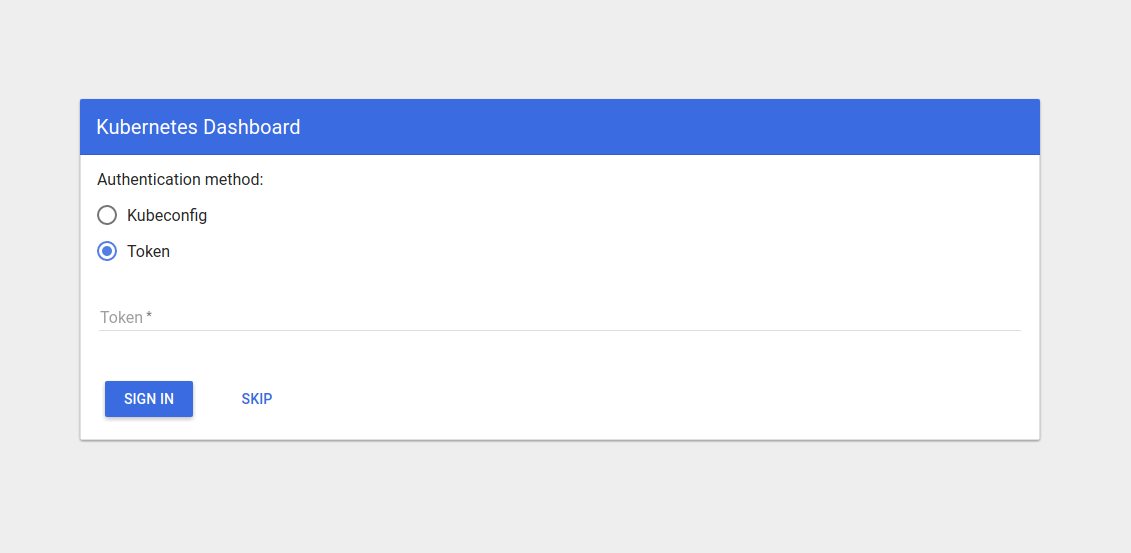
\includegraphics[width=5.20833in,height=2.5in]{assets/dashboard-login-old.png}\\
Od 29 stycznia 2018 roku widzę poprawny ekran logowania (opcja Basic):

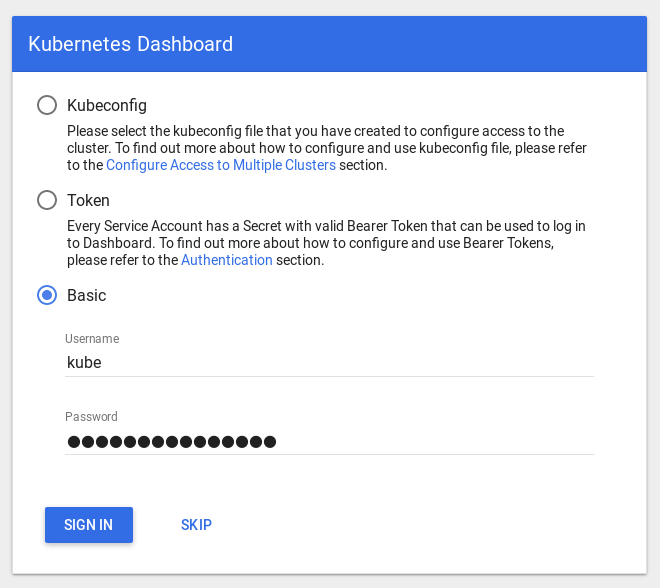
\includegraphics[width=5.20833in,height=4.63542in]{assets/dashboard-login-new.png}\\

\hypertarget{instalacja-dodatkowych-aplikacji-z-uux17cyciem-kubespray}{%
\subsubsection{Instalacja dodatkowych aplikacji z użyciem
Kubespray}\label{instalacja-dodatkowych-aplikacji-z-uux17cyciem-kubespray}}

\passthrough{\lstinline!Kubespray!} ma wbudowaną instalację kilku
dodatkowych aplikacji playbookiem
\passthrough{\lstinline!upgrade-cluster.yml!} z tagiem
\passthrough{\lstinline!apps!} (skrypt
\passthrough{\lstinline!bin/setup-cluster-upgrade!}).

Zmieniłem~\passthrough{\lstinline!kube\_script\_dir!} na lokalizacje z
poza \passthrough{\lstinline!/usr/local/bin!}, bo w systemie
\passthrough{\lstinline!CoreOS!} jest read-only squashfsem, wybrałem
\passthrough{\lstinline!/opt/bin!} ponieważ znajdował się już~w
\passthrough{\lstinline!PATHie!} na \passthrough{\lstinline!CoreOS!}.
Później dowiedziałem się, że domyślnie zmiany
\passthrough{\lstinline!CoreOS!} powinny być umieszczane w folderze
\passthrough{\lstinline!/opt!}

W końcu ze względu na liczne błędy zarzuciłem temat.

\hypertarget{instalacja-helm}{%
\subsubsection{Instalacja Helm}\label{instalacja-helm}}

\href{https://github.com/kubernetes/helm}{\passthrough{\lstinline!Helm!}}
jest menadżerem pakietów dla \passthrough{\lstinline!k8s!}. Jego głównym
zadaniem jest standaryzacja, automatyzacja i ułatwienie instalacji
aplikacji w \passthrough{\lstinline!k8s!}.

\passthrough{\lstinline!Helm!} składa się z:

\begin{itemize}
\tightlist
\item
  programu \passthrough{\lstinline!helm!} uruchamianego lokalnie i
  korzystającego z danych dostępowych
  \passthrough{\lstinline!kubectla!},
\item
  aplikacji serwerowej \passthrough{\lstinline!Tiller!}, z którą
  \passthrough{\lstinline!helm!} prowadzi interakcje,
\item
  pakietów \passthrough{\lstinline!Charts!} i ich repozytoriów,
  domyślnie jest to
  \href{https://github.com/kubernetes/charts}{\passthrough{\lstinline!kubernetes/charts!}},
\end{itemize}

Jego instalacja sprowadza się~do:

\begin{enumerate}
\def\labelenumi{\arabic{enumi}.}
\tightlist
\item
  ściągnięcia pliku wykonywalnego dla obecnej architektury,
\item
  dodania roli RBAC dla \passthrough{\lstinline!Tillera!},
\item
  Wywołanie komendy
  \passthrough{\lstinline!helm init --service-account tiller!}
\end{enumerate}

Wszystkie kroki zawierają się w skrypcie
\passthrough{\lstinline!bin/install-helm!}. Ze względu na braku
dystrybucji \passthrough{\lstinline!Helm!} na
\passthrough{\lstinline!FreeBSD!} całość uruchamiam przez SSH na
węźle-zarządcy (domyślnie \passthrough{\lstinline!s4!}).

Szybko okazało się, że większość pakietów wymaga trwałych zasobów
dyskowych i nie uda się ich uruchomić bez ich konfiguracji w sieci
uczelnianej.

\hypertarget{docelowa-konfiguracja-w-sieci-uczelnianej}{%
\chapter{Docelowa konfiguracja w sieci
uczelnianej}\label{docelowa-konfiguracja-w-sieci-uczelnianej}}

Pełną konfiguracja \passthrough{\lstinline!k8s!} można uruchomić z
maszyny ldap; znajduje się ona w folderze
\passthrough{\lstinline!/pub/Linux/CoreOS/zetis/kubernetes!} maszyny
\passthrough{\lstinline!ldap!}, który zawiera podane foldery:

\begin{itemize}
\tightlist
\item
  \passthrough{\lstinline!kubernetes-cluster!} - moje repozytorium
  zawierające konfigurację i skrypty pozwalające uruchomić klaster,
\item
  \passthrough{\lstinline!boot!} - skrót do folderu
  \passthrough{\lstinline!kubernetes-cluster/zetis/WWW/boot!}
  zawierającego konfigurację iPXE oraz Ignition:

  \begin{itemize}
  \tightlist
  \item
    \passthrough{\lstinline!coreos.ign!} - plik konfigurujący CoreOS,
    wygenerowany z pliku \passthrough{\lstinline!coreos.yml!} narzędziem
    do transpilacji konfiguracji
    \href{https://github.com/coreos/container-linux-config-transpiler}{\passthrough{\lstinline!ct!}},
    narzędzie domyślnie nie jest skompilowane na FreeBSD i musimy
    uruchomić je z Linuxa,
  \end{itemize}
\item
  \passthrough{\lstinline!log!} - standardowe wyjście uruchamianych
  komend,
\end{itemize}

\hypertarget{procedura-uruchomienia-klastra}{%
\section{Procedura uruchomienia
klastra}\label{procedura-uruchomienia-klastra}}

\begin{enumerate}
\def\labelenumi{\arabic{enumi}.}
\tightlist
\item
  Wchodzę na maszynie \passthrough{\lstinline!ldap!} do folderu
  \passthrough{\lstinline!/pub/Linux/CoreOS/zetis/kubernetes/kubernetes-cluster!}
\item
  Upewniam się, że mój klucz SSH znajduje się w
  \passthrough{\lstinline!boot/coreos.ign!},
\item
  Włączam maszyny-węzły wybierając z menu
  \passthrough{\lstinline!iPXE CoreOS!} -\textgreater{}
  \passthrough{\lstinline!k8s!} lub wybierając w narzędziu
  \passthrough{\lstinline!boot!} bezpośrednio
  \passthrough{\lstinline!coreos kub!},
\item
  Upewniam się, że mam bezhasłowy dostęp do tych maszyn, minimalna
  konfiguracja \passthrough{\lstinline!\~/.ssh/config!} to:
\end{enumerate}

\begin{lstlisting}
Host s?
  User admin
  StrictHostKeyChecking no
  UserKnownHostsFile /dev/null

Host *
  IdentityFile ~/.ssh/id_rsa
  IdentitiesOnly yes
\end{lstlisting}

\begin{enumerate}
\def\labelenumi{\arabic{enumi}.}
\setcounter{enumi}{4}
\tightlist
\item
  Upewniam się, że istnieje folder
  \passthrough{\lstinline!kubespray/my\_inventory!}, jeżeli nie, to go
  tworzymę kopiując domyślną konfigurację:
\end{enumerate}

\begin{lstlisting}
cp -rav kubespray/inventory kubespray/my_inventory
\end{lstlisting}

\begin{enumerate}
\def\labelenumi{\arabic{enumi}.}
\setcounter{enumi}{5}
\tightlist
\item
  Otwieram plik \passthrough{\lstinline!inventory/inventory.cfg!} i
  upewniam się, że uruchomione maszyny są obecne w sekcji
  \passthrough{\lstinline![all]!} oraz przypisane do odpowiednich ról:
  \passthrough{\lstinline![kube-master]!} i
  \passthrough{\lstinline![etcd]!} lub
  \passthrough{\lstinline![kube-node]!}. Identyfikatorem maszyny jest
  pierwsze słowo w grupie \passthrough{\lstinline![all]!}, przykładowa
  konfiguracja dla maszyn \passthrough{\lstinline!s4!},
  \passthrough{\lstinline!s5!} i \passthrough{\lstinline!s6!} z jednym
  zarządcą to:
\end{enumerate}

\begin{lstlisting}
[all]
;s3  ip=10.146.225.3
s4  ip=10.146.225.4
s5  ip=10.146.225.5
s6  ip=10.146.225.6
;s7  ip=10.146.225.7
;s8  ip=10.146.225.8
;s9  ip=10.146.225.9
;sa  ip=10.146.225.10
;sb  ip=10.146.225.11
;sc  ip=10.146.225.12

[kube-master]
s4

[kube-node]
s5
s6

[etcd]
s4

[k8s-cluster:children]
kube-node
kube-master
\end{lstlisting}

Opcjonalnie można do każdego węzła:

\begin{itemize}
\tightlist
\item
  dopisać
  \passthrough{\lstinline!ansible\_python\_interpreter=/opt/bin/python!},
  żeby ułatwić uruchamianie ansibla partiami,
\item
  dopisać
  \passthrough{\lstinline!ansible\_host=<prawdziwa\_nazwa\_hosta>!},
  jeżeli che się korzystać z pierwszego wyrazu opisu węzła jako aliasu,
  a nie faktycznej jego nazwy w sieci uczelnianej,
\end{itemize}

\begin{enumerate}
\def\labelenumi{\arabic{enumi}.}
\setcounter{enumi}{6}
\tightlist
\item
  Upewniam się, że plik
  \passthrough{\lstinline!inventory/group\_vars/all.yml!} zawiera naszą
  konfigurację; minimalny przykład:
\end{enumerate}

\begin{lstlisting}
cluster_name: zetis-kubernetes
bootstrap_os: coreos
kube_basic_auth: true
kubeconfig_localhost: true
kubectl_localhost: true
download_run_once: true
cert_management: "{{ 'vault' if groups.get('vault', None) else 'script' }}"
helm_enabled: true
helm_deployment_type: docker
kube_script_dir: /opt/bin/kubernetes-scripts
\end{lstlisting}

\begin{enumerate}
\def\labelenumi{\arabic{enumi}.}
\setcounter{enumi}{7}
\tightlist
\item
  Uruchamiam konfigurowanie maszyn
  \passthrough{\lstinline!bin/setup-cluster!} lub bez skryptu:
\end{enumerate}

\begin{lstlisting}[language=bash]
ldap% cd kubespray
ldap% ansible-playbook -i my_inventory/inventory.cfg cluster.yml -b -v
\end{lstlisting}

Po około 10-20 minutach skrypt powinien zakończyć się wpisami pokroju:

\begin{lstlisting}
...
PLAY RECAP ********
localhost                  : ok=2    changed=0    unreachable=0    failed=0   
s4                         : ok=281  changed=94   unreachable=0    failed=0   
s5                         : ok=346  changed=80   unreachable=0    failed=0   
s6                         : ok=186  changed=54   unreachable=0    failed=0   
...
\end{lstlisting}

\begin{enumerate}
\def\labelenumi{\arabic{enumi}.}
\setcounter{enumi}{8}
\tightlist
\item
  Weryfikuję instalację:
\end{enumerate}

\begin{lstlisting}[language=bash]
ldap% bin/kubectl get nodes
NAME      STATUS    ROLES     AGE       VERSION
s4        Ready     master    2m        v1.9.1_coreos.0
s5        Ready     node      2m        v1.9.1_coreos.0
s6        Ready     node      2m        v1.9.1_coreos.0
\end{lstlisting}

\hypertarget{sprawdzanie-czy-klaster-dziaux142a}{%
\section{Sprawdzanie, czy klaster
działa}\label{sprawdzanie-czy-klaster-dziaux142a}}

Wywołanie skryptu \passthrough{\lstinline!bin/students nazarewk create!}
jest równoważne uruchomieniu komendy
\passthrough{\lstinline!kubectl create -f nazarewk.yml!}, gdzie plik
\passthrough{\lstinline!nazarewk.yml!} to:

\begin{lstlisting}
apiVersion: v1
kind: Namespace
metadata:
  name: nazarewk
  labels:
    name: nazarewk
---
apiVersion: v1
kind: ServiceAccount
metadata:
  name: nazarewk
  namespace: nazarewk
---
kind: RoleBinding
apiVersion: rbac.authorization.k8s.io/v1
metadata:
  name: nazarewk-admin-binding
  namespace: nazarewk
roleRef:
  kind: ClusterRole
  name: admin
  apiGroup: rbac.authorization.k8s.io
subjects:
- kind: ServiceAccount
  name: nazarewk
\end{lstlisting}

W skrócie:

\begin{itemize}
\tightlist
\item
  tworzę \passthrough{\lstinline!Namespace!}
\item
  tworzę \passthrough{\lstinline!ServiceAccount!}
\item
  przypisuję wbudowaną \passthrough{\lstinline!Role!} o nazwie
  \passthrough{\lstinline!admin!} do
  \passthrough{\lstinline!ServiceAccount!} o nazwie
  \passthrough{\lstinline!nazarewk!} za pomocą
  \passthrough{\lstinline!RoleBinding!},
\end{itemize}

\hypertarget{korzystanie-z-klastra-jako-student}{%
\subsubsection{Korzystanie z klastra jako
student}\label{korzystanie-z-klastra-jako-student}}

\begin{itemize}
\tightlist
\item
  tworzę użytkownika z jego własnym \passthrough{\lstinline!Namespace!}
\end{itemize}

\begin{lstlisting}
ldap% bin/students nazarewk create
namespace "nazarewk" created
serviceaccount "nazarewk" created
rolebinding "nazarewk-admin-binding" created
Tokens:
eyJhb<<<SKROCONY TOKEN>>>ahHfxU-TRw
ldap% bin/students
NAME          STATUS    AGE
default       Active    3m
kube-public   Active    3m
kube-system   Active    3m
nazarewk      Active    16s
\end{lstlisting}

\begin{itemize}
\tightlist
\item
  kopiuję token na \passthrough{\lstinline!s2!} z uruchomionym ubuntu:
\end{itemize}

\begin{lstlisting}
  ldap% bin/student-tokens nazarewk | ssh nazarewk@s2 "cat > /tmp/token"
\end{lstlisting}

\begin{itemize}
\tightlist
\item
  pobieram \passthrough{\lstinline!kubectl!}
\end{itemize}

\begin{lstlisting}
s2% cd /tmp
s2% curl -LO https://storage.googleapis.com/kubernetes-release/release/$(curl -s https://storage.googleapis.com/kubernetes-release/release/stable.txt)/bin/linux/amd64/kubectl
s2% chmod +x kubectl
s2% sudo mv kubectl /usr/local/bin
s2% source <(kubectl completion zsh)
\end{lstlisting}

\begin{itemize}
\tightlist
\item
  sprawdzam, czy mam dostęp do klastra
\end{itemize}

\begin{lstlisting}
s2% kubectl get nodes
The connection to the server localhost:8080 was refused - did you specify the right host or port?
\end{lstlisting}

\begin{itemize}
\tightlist
\item
  konfiguruję kubectl (najprościej aliasem)
\end{itemize}

\begin{lstlisting}
s2% alias kubectl='command kubectl -s "https://s4:6443" --insecure-skip-tls-verify=true --token="$(cat /tmp/token)" -n nazarewk'
\end{lstlisting}

\begin{itemize}
\tightlist
\item
  weryfikuję brak dostępu do zasobów globalnych
\end{itemize}

\begin{lstlisting}
s2% kubectl get nodes
Error from server (Forbidden): nodes is forbidden: User "system:serviceaccount:nazarewk:nazarewk" cannot list nodes at the cluster scope
\end{lstlisting}

\begin{itemize}
\tightlist
\item
  tworzę deployment z przykładową aplikacją
\end{itemize}

\begin{lstlisting}
s2% kubectl run echoserver --image=gcr.io/google_containers/echoserver:1.4 --port=8080 --replicas=2
deployment "echoserver" created
\end{lstlisting}

\begin{lstlisting}
s2% kubectl get deployments
NAME         DESIRED   CURRENT   UP-TO-DATE   AVAILABLE   AGE
echoserver   2         2         2            2           3m
\end{lstlisting}

\begin{lstlisting}
s2% kubectl get pods
NAME                         READY     STATUS    RESTARTS   AGE
echoserver-7b9bbf6ff-22df4   1/1       Running   0          4m
echoserver-7b9bbf6ff-c6kbv   1/1       Running   0          4m
\end{lstlisting}

\begin{itemize}
\tightlist
\item
  wystawiam port, żeby dostać się do aplikacji spoza klastra
\end{itemize}

\begin{lstlisting}
s2% kubectl expose deployment echoserver --type=NodePort
service "echoserver" exposed
\end{lstlisting}

\begin{lstlisting}
s2% kubectl describe services/echoserver | grep -e NodePort:
NodePort:                 <unset>  30100/TCP
\end{lstlisting}

\begin{lstlisting}
s2% curl s4:30100
CLIENT VALUES:
client_address=10.233.107.64
command=GET
real path=/
query=nil
request_version=1.1
request_uri=http://s4:8080/

SERVER VALUES:
server_version=nginx: 1.10.0 - lua: 10001

HEADERS RECEIVED:
accept=*/*
host=s4:30100
user-agent=curl/7.47.0
BODY:
-no body in request-
\end{lstlisting}

\begin{itemize}
\tightlist
\item
  sprawdzam, czy z \passthrough{\lstinline!ldapa!} też mam dostęp do
  aplikacji:
\end{itemize}

\begin{lstlisting}
ldap% curl s4:30100
CLIENT VALUES:
client_address=10.233.107.64
command=GET
real path=/
query=nil
request_version=1.1
request_uri=http://s4:8080/

SERVER VALUES:
server_version=nginx: 1.10.0 - lua: 10001

HEADERS RECEIVED:
accept=*/*
host=s4:30100
user-agent=curl/7.58.0
BODY:
-no body in request-
\end{lstlisting}

\begin{itemize}
\tightlist
\item
  usuwam użytkownika
\end{itemize}

\begin{lstlisting}
ldap% bin/students nazarewk delete
namespace "nazarewk" deleted
serviceaccount "nazarewk" deleted
rolebinding "nazarewk-admin-binding" deleted
Tokens:
Error from server (NotFound): serviceaccounts "nazarewk" not found
\end{lstlisting}

\begin{itemize}
\tightlist
\item
  sprawdzam, czy coś zostało po koncie użytkownika
\end{itemize}

\begin{lstlisting}
ldap% curl s4:30100
curl: (7) Failed to connect to s4 port 30100: Connection refused
\end{lstlisting}

\begin{lstlisting}
ldap% bin/kubectl get namespace 
NAME          STATUS    AGE
default       Active    46m
kube-public   Active    46m
kube-system   Active    46m
\end{lstlisting}

\hypertarget{rezultaty-i-wnioski}{%
\chapter{Rezultaty i wnioski}\label{rezultaty-i-wnioski}}

Główne założenia pracy inżynierskiej zostały spełnione. Wyjaśniłem dużą
ilość zagadnień związanych z \passthrough{\lstinline!k8s!} oraz oddałem
do użytku skrypty konfigurujące klaster \passthrough{\lstinline!k8s!}
wraz z prostym w obsłudze dodawaniem i usuwaniem jego użytkowników.

W trakcie pisania pracy temat okazał się zbyt obszerny, żeby go
kompletnie i wyczerpująco opisać w pracy inżynierskiej. W związku z tym
musiałem wybrać tylko najważniejsze informacje i przekazać je w możliwie
najkrótszej formie.

Projekt jest bardzo aktywnie rozwijany, więc wiele informacji wyszło na
jaw w końcowych etapach pisania pracy. W samej pracy pojawiły się
jedynie wzmianki o nich bez dogłębnej analizy.

Nie udało mi się przeprowadzić~testów wydajnościowych klastra ze względu
na brak czasu.

\appendix

\hypertarget{przypisy}{%
\chapter{Przypisy}\label{przypisy}}

\theendnotes

\hypertarget{wykaz-skryptuxf3w}{%
\chapter{Wykaz skryptów}\label{wykaz-skryptuxf3w}}

\hypertarget{repozytorium-kubernetes-cluster}{%
\section{repozytorium
kubernetes-cluster}\label{repozytorium-kubernetes-cluster}}

\passthrough{\lstinline!kubernetes-cluster!}
(\passthrough{\lstinline!https://github.com/nazarewk/kubernetes-cluster!})
jest repozytorium Git, które zawiera kompletny kod źródłowy
wykorzystywany w tej pracy inżynierskiej.

Kod można znaleźć~i uruchomić w sieci uczelnianej z katalogu
\passthrough{\lstinline!/pub/Linux/CoreOS/zetis/kubernetes/kubernetes-cluster/!}
na maszynie \passthrough{\lstinline!ldap!}.

\hypertarget{binpull}{%
\subsubsection{bin/pull}\label{binpull}}

Pobiera aktualną wersję~repozytorium wraz z najnowszą wersją zależności:

\begin{lstlisting}[language=bash]
#!/bin/sh
# Author: Krzysztof Nazarewski <nazarewk@gmail.com>
# Purpose: git pull wrapper including submodule updates

git pull || (git fetch --all && git reset --hard origin)
git submodule update --init --remote --recursive
chmod +x ${0%/*}/*
\end{lstlisting}

\hypertarget{binvars}{%
\subsubsection{bin/vars}\label{binvars}}

Zawiera wspólne zmienne środowiskowe wykorzystywane w reszcie skryptów
oraz linii komend:

\begin{lstlisting}[language=bash]
#!/bin/sh
# Author: Krzysztof Nazarewski <nazarewk@gmail.com>
# Purpose: Holds common variables used in all other scripts

if [ -z "$KC_CONFIGURED" ]; then
  KC_CONFIGURED=1

  BIN="$(realpath ${0%/*})"
  PATH="$BIN:$PATH"
  PDIR="${BIN%/*}"
  VENV="$PDIR/.env"
  KUBESPRAY="$PDIR/kubespray"
  INVENTORY="$KUBESPRAY/my_inventory"
  CONFIG_FILE="$INVENTORY/inventory.cfg"

  export KUBECONFIG="$KUBESPRAY/artifacts/admin.conf"
  export ANSIBLE_CONFIG="$PDIR/ansible.cfg"
fi
\end{lstlisting}

\hypertarget{binensure-virtualenv}{%
\subsubsection{bin/ensure-virtualenv}\label{binensure-virtualenv}}

Konfiguruje środowisko Pythona, włącznie z próbą instalacji brakującego
\passthrough{\lstinline!virtualenv!} przez
\passthrough{\lstinline!apt!}:

\begin{lstlisting}[language=bash]
#!/bin/sh
# Author: Krzysztof Nazarewski <nazarewk@gmail.com>
# Purpose: installs python virtualenv

. ${0%/*}/vars
python="$(which python)"
activate="$VENV/bin/activate"

find_virtualenv() {
    which virtualenv 2> /dev/null || which virtualenv
}

install_virtualenv () {
  # Installs pip and/or virtualenv

  local pip=$(which pip)
  local apt=$(which apt)
  if [ ! -z "$pip" ]; then
    sudo $pip install virtualenv
    return 0
  elif [ ! -z "$apt" ]; then
    sudo $apt install virtualenv
    return 0
  else
    echo 'Virtualenv, pip and apt-get are both missing, cannot proceed'
    exit 1
  fi
}

create_env () {
    local cmd=$(find_virtualenv)
    [ -z "$cmd" ] && install_virtualenv && cmd=$(find_virtualenv)

    $cmd -p $python $VENV
    . $activate

    pip install -U pip setuptools
}

[ -z "$python" ] && echo 'python is missing' && exit 1
[ -e "$activate" ] && . $activate || create_env
pip install -U -r $PDIR/requirements.txt
\end{lstlisting}

\hypertarget{binensure-configuration}{%
\subsubsection{bin/ensure-configuration}\label{binensure-configuration}}

Generuje brakujące pliki konfiguracyjne SSH,
\passthrough{\lstinline!inventory.cfg!} i
\passthrough{\lstinline!group\_vars/all.yml!} nie nadpisując
istniejących:

\begin{lstlisting}[language=bash]
#!/bin/sh
# Author: Krzysztof Nazarewski <nazarewk@gmail.com>
# Purpose: configures cluster (SSH, inventory, group_vars)

. ${0%/*}/vars
SSH_CFG_DST="$HOME/.ssh/config"
SSH_CFG="$PDIR/zetis/.ssh/kubernetes.conf"


is_ssh_config_missing () {
  cat << EOF | python
import sys
expected = open('$SSH_CFG', 'rb').read()
existing = open('$SSH_CFG_DST', 'rb').read()
sys.exit(expected in existing)
EOF
  return $?
}

is_ssh_config_missing && cat $SSH_CFG >> $SSH_CFG_DST

file="$INVENTORY/inventory.cfg"
[ -f "$file" ] || cat << EOF > "$file"
[all]
;s3  ip=10.146.225.3
s4  ip=10.146.225.4
s5  ip=10.146.225.5
s6  ip=10.146.225.6
;s7  ip=10.146.225.7
;s8  ip=10.146.225.8
;s9  ip=10.146.225.9
;sa  ip=10.146.225.10
;sb  ip=10.146.225.11
;sc  ip=10.146.225.12

[kube-master]
s4

[kube-node]
s5
s6

[etcd]
s4

[k8s-cluster:children]
kube-node
kube-master
EOF

file="$INVENTORY/group_vars/all.yml"
[ -f "$file" ] || cat << EOF > "$file"
cluster_name: zetis-kubernetes
bootstrap_os: coreos
kube_basic_auth: true
kubeconfig_localhost: true
kubectl_localhost: true
download_run_once: true
cert_management: "{{ 'vault' if groups.get('vault', None) else 'script' }}"
helm_enabled: true
helm_deployment_type: docker
kube_script_dir: /opt/bin/kubernetes-scripts
EOF
\end{lstlisting}

\hypertarget{binrender-coreos}{%
\subsubsection{bin/render-coreos}\label{binrender-coreos}}

Generuje konfigurację Ignition (JSON) na podstawie Container Linux
Config (YAML):

\begin{lstlisting}[language=bash]
#!/bin/sh
# Author: Krzysztof Nazarewski <nazarewk@gmail.com>
# Purpose: renders CoreOS Ignition (incl. retrieving binary)

. ${0%/*}/vars
ct_version=${1:-0.6.1}
boot="$PDIR/zetis/WWW/boot"
url='https://github.com/coreos/container-linux-config-transpiler'
url="$url/releases/download"
url="$url/v${ct_version}/ct-v${ct_version}-x86_64-unknown-linux-gnu"

wget -nc $url -O $BIN/ct
chmod +x $BIN/ct
$BIN/ct -pretty \
  -in-file "$boot/coreos.yml" \
  -out-file "$boot/coreos.ign"
\end{lstlisting}

\hypertarget{binsetup-cluster}{%
\subsubsection{bin/setup-cluster}\label{binsetup-cluster}}

Właściwy skrypt konfigurujący klaster na działających maszynach CoreOS:

\begin{lstlisting}[language=bash]
#!/bin/sh
# Author: Krzysztof Nazarewski <nazarewk@gmail.com>
# Purpose: sets up the cluster

. ${0%/*}/vars
. $BIN/ensure-configuration
. $BIN/activate

(
  cd $KUBESPRAY;
  ansible-playbook -i $INVENTORY/inventory.cfg cluster.yml -b -v $@
)

chmod -R 700 $KUBESPRAY/{artifacts/admin.conf,credentials}

cat << EOF
Login credentials:
  user: kube
  password: $(cat $PDIR/credentials/kube_user)
EOF
\end{lstlisting}

\hypertarget{binsetup-cluster-full}{%
\subsubsection{bin/setup-cluster-full}\label{binsetup-cluster-full}}

Skrót do pobierania najnowszej wersji, a następnie uruchamiania klastra:

\begin{lstlisting}[language=bash]
#!/bin/sh
. ${0%/*}/vars

$BIN/pull
$BIN/setup-cluster $@
\end{lstlisting}

\hypertarget{binsetup-cluster-upgrade}{%
\subsubsection{bin/setup-cluster-upgrade}\label{binsetup-cluster-upgrade}}

Skrypt analogiczny do \passthrough{\lstinline!setup-cluster!}, ale
wywołujący \passthrough{\lstinline!upgrade-cluster.yml!} zamiast
\passthrough{\lstinline!cluster.yml!}:

\begin{lstlisting}[language=bash]
#!/bin/sh
# Author: Krzysztof Nazarewski <nazarewk@gmail.com>
# Purpose: runs upgrade-cluster.yml instead of cluster.yml

. ${0%/*}/vars
. $BIN/ensure-configuration
. $BIN/activate

cd $KUBESPRAY
ansible-playbook -i $INVENTORY/inventory.cfg upgrade-cluster.yml -b -v $@
\end{lstlisting}

\hypertarget{binkubectl}{%
\subsubsection{bin/kubectl}\label{binkubectl}}

Skrót \passthrough{\lstinline!kubectl!} z automatycznym dołączaniem
konfiguracji \passthrough{\lstinline!kubespray!}:

\begin{lstlisting}[language=bash]
#!/bin/sh
# Author: Krzysztof Nazarewski <nazarewk@gmail.com>
# Purpose: kubectl wrapper which uses generated  configurations

# Handle running kubectl from PATH
[ "${0%/*}" == "$0" ] \
 && _bin=$(dirname $(which kubectl)) \
 || _bin=${0%/*}

. $_bin/vars

local_bin="$PDIR/artifacts/kubectl"

if [ -f $local_bin ]; then
  chmod +x $local_bin
  kubectl=$local_bin
else
  kubectl=/usr/bin/kubectl
fi

$kubectl $@
\end{lstlisting}

\hypertarget{binstudents}{%
\subsubsection{bin/students}\label{binstudents}}

Skrypt zarządzający obiektami \passthrough{\lstinline!k8s!}
użytkowników, czyli studentów:

\begin{lstlisting}[language=bash]
#!/bin/sh
# Author: Krzysztof Nazarewski <nazarewk@gmail.com>
# Purpose: executes operations on users (create, get, describe, delete)

. ${0%/*}/vars

kubectl_command () {
local users="$1"
local cmd="$2"
for name in $users; do
  cat  <<EOF | $BIN/kubectl $cmd -f -
apiVersion: v1
kind: Namespace
metadata:
  name: ${name}
  labels:
    name: ${name}

---

apiVersion: v1
kind: ServiceAccount
metadata:
  name: ${name}
  namespace: ${name}

---

kind: RoleBinding
apiVersion: rbac.authorization.k8s.io/v1
metadata:
  name: ${name}-admin-binding
  namespace: ${name}
roleRef:
  kind: ClusterRole
  name: admin
  apiGroup: rbac.authorization.k8s.io
subjects:
- kind: ServiceAccount
  name: ${name}
EOF
  echo Tokens:
  $BIN/student-tokens ${name}
done
}

case $1 in
  ""|list)
    $BIN/kubectl get namespace
    ;;
  -h)
    cat << EOF
    Usage: $0 "<usernames>" create|get|describe|delete
      where <usernames> is a single-argument list of usernames
    You can also call it without arguments to list users (namespaces)
EOF
    ;;
  *)
    kubectl_command "$@"
    ;;
esac
\end{lstlisting}

\hypertarget{binstudent-tokens}{%
\subsubsection{bin/student-tokens}\label{binstudent-tokens}}

Listuje przepustki konkretnego użytkownika:

\begin{lstlisting}[language=bash]
#!/bin/sh
# Author: Krzysztof Nazarewski <nazarewk@gmail.com>
# Purpose: lists kubernetes authentication tokens for specified user

. ${0%/*}/vars
name=$1
args="--namespace $name get serviceaccount $name"
args="$args -o jsonpath={.secrets[*].name}"
for token in `$BIN/kubectl $args`; do
    args="get secrets $token --namespace $name"
    args="$args  -o jsonpath={.data.token}"
    $BIN/kubectl $args | base64 --decode
    echo
done
\end{lstlisting}

\hypertarget{bininstall-helm}{%
\subsubsection{bin/install-helm}\label{bininstall-helm}}

Instaluje menadżer pakietów \passthrough{\lstinline!Helm!}:

\begin{lstlisting}[language=bash]
#!/bin/sh
# Author: Krzysztof Nazarewski <nazarewk@gmail.com>
# Purpose: installs helm package manager into Kubernetes cluster

. ${0%/*}/vars

host=${1:-s4}

ssh () {
  command ssh $host sudo $@
}

cat <<EOF | ssh bash
export HELM_INSTALL_DIR=/opt/bin
url='https://raw.githubusercontent.com/kubernetes/helm/master/scripts/get'
[ -f /opt/bin/helm ] || curl \$url | bash
EOF

cat <<EOF | ssh kubectl create -f -
apiVersion: v1
kind: ServiceAccount
metadata:
  name: tiller
  namespace: kube-system
---
apiVersion: rbac.authorization.k8s.io/v1beta1
kind: ClusterRoleBinding
metadata:
  name: tiller
roleRef:
  apiGroup: rbac.authorization.k8s.io
  kind: ClusterRole
  name: cluster-admin
subjects:
  - kind: ServiceAccount
    name: tiller
    namespace: kube-system
EOF

ssh helm version | grep Server: || ssh helm init --service-account tiller
\end{lstlisting}

\hypertarget{zetis.sshkubernetes.conf}{%
\subsubsection{zetis/.ssh/kubernetes.conf}\label{zetis.sshkubernetes.conf}}

Częściowy plik konfiguracyjny SSH do umieszczenia w
\passthrough{\lstinline!\~/.ssh/config!}:

\begin{lstlisting}[language=bash]
Host s?
  User admin

IdentityFile ~/.ssh/id_rsa
IdentitiesOnly yes

Host s?
  StrictHostKeyChecking no
  UserKnownHostsFile /dev/null
\end{lstlisting}

\hypertarget{zetiswwwbootcoreos.ipxe}{%
\subsubsection{zetis/WWW/boot/coreos.ipxe}\label{zetiswwwbootcoreos.ipxe}}

Skrypt iPXE uruchamiający maszynę z CoreOS:

\begin{lstlisting}[language=bash]
#!ipxe
set ftp http://ftp/pub/

set base-url ${ftp}/Linux/CoreOS/alpha
set ignition ${ftp}/Linux/CoreOS/zetis/kubernetes/boot/coreos.ign

set opts ${opts} coreos.autologin
set opts ${opts} coreos.first_boot=1 coreos.config.url=${ignition}
set opts ${opts} systemd.journald.max_level_console=debug
kernel ${base-url}/coreos_production_pxe.vmlinuz ${opts}
initrd ${base-url}/coreos_production_pxe_image.cpio.gz

boot
\end{lstlisting}

\hypertarget{zetiswwwbootcoreos.yml}{%
\subsubsection{zetis/WWW/boot/coreos.yml}\label{zetiswwwbootcoreos.yml}}

Plik konfiguracyjny Container Linux Config w formacie YAML, docelowo do
przepuszczenia przez narzędzie \passthrough{\lstinline!ct!}. Wyjątkowo
skróciłem ten skrypt, ze względu na długość kluczy SSH:

\begin{lstlisting}
passwd:
  users:
  - name: admin
    groups: [sudo, docker]
    ssh_authorized_keys:
    - ssh-rsa <klucz RSA> ato@volt.iem.pw.edu.pl
    - ssh-rsa <klucz RSA> nazarewk
    - ssh-rsa <klucz RSA> nazarewk@ldap.iem.pw.edu.pl
\end{lstlisting}

\hypertarget{zetiswwwbootcoreos.ign}{%
\subsubsection{zetis/WWW/boot/coreos.ign}\label{zetiswwwbootcoreos.ign}}

Z powyższego pliku wygenerowany zostaje (również skrócony) plik JSON:

\begin{lstlisting}
{
  "ignition": {
    "config": {},
    "timeouts": {},
    "version": "2.1.0"
  },
  "networkd": {},
  "passwd": {
    "users": [
      {
        "groups": [
          "sudo",
          "docker"
        ],
        "name": "admin",
        "sshAuthorizedKeys": [
          "ssh-rsa <klucz RSA> nazarewk",
          "ssh-rsa <klucz RSA> nazarewk@ldap.iem.pw.edu.pl",
          "ssh-rsa <klucz RSA> ato@volt.iem.pw.edu.pl"
        ]
      }
    ]
  },
  "storage": {},
  "systemd": {}
}
\end{lstlisting}

\hypertarget{repozytorium-ipxe-boot}{%
\section{repozytorium ipxe-boot}\label{repozytorium-ipxe-boot}}

\passthrough{\lstinline!ipxe-boot!}
(\passthrough{\lstinline!https://github.com/nazarewk/ipxe-boot!}) jest
repozytorium kodu umożliwiającego uruchomienie środowiska bezdyskowego
poza uczelnią.

Repozytorium nie zostało wykorzystane w finalnej konfiguracji, więc nie
będę opisywał jego zawartości.
\end{document}
